\documentclass[a4paper,12pt]{article}

% Module de base utf, français
\usepackage[utf8]{inputenc}
\usepackage[T1]{fontenc}
\usepackage[french]{babel}
% gestion des marges
\usepackage[top=2cm, bottom=2cm, left=2cm, right=2cm]{geometry}

% quote
% \usepackage{csquotes}

% Packages math
%\usepackage{amsmath}
%\usepackage{amssymb}
%\usepackage{mathrsfs}

% Package tableau
\usepackage{multirow}

% Package insertion d'image
\usepackage{graphicx}
\usepackage{float}
\usepackage{subcaption} %image multiple

% Package url
\usepackage{url}	

% Package de couleur
\usepackage{color}
\usepackage[colorlinks,linkcolor=black,urlcolor=blue]{hyperref}

% Package pour le code, nécessite package color
\usepackage{listings}
\usepackage{amsmath}
\lstset{ % General setup for the package
	language=Python,
	basicstyle=\small\sffamily,
	numbers=left,
 	numberstyle=\tiny,
	frame=tb,
	tabsize=4,
	columns=fixed,
	showstringspaces=false,
	showtabs=false,
	keepspaces,
	commentstyle=\color{red},
	keywordstyle=\color{blue},
	breaklines=true
}

% Packages Verbatim
\usepackage{moreverb}

% nouvelle commande pour ~
%\newcommand{\tidle}{\char`\~}

\title{Projet L3\\Ingénierie des langues\\Fouille de données}
\author{GOEHRY Martial\\16711476}

\begin{document}
	\maketitle
	\tableofcontents
	\newpage
	
\section*{Introduction}
	Ce projet a pour but de développer un modèle permettant de catégoriser des emails en spam ou ham.
	La définition d'un spam dans le dictionnaire \emph{Larousse} est:
	
	\begin{quote}
	"Courrier électronique non sollicité envoyé en grand nombre à des boîtes aux lettres électroniques ou à des forums, dans un but publicitaire ou commercial."
	\end{quote}
	
	Il est possible d'ajouter à cette catégorie tous les mails indésirables comme les tentatives d'hameçonnage permettant de soutirer des informations personnelles à une cible.\\ 
	
	L'objectif est de travailler uniquement sur les données textuelles issues du corps du mail.
	Nous avons donc comme point de départ les éléments suivants:
	\begin{itemize}
		\item langue: anglais
		\item corpus: monolingue écrit
		\item type: e-mail
	\end{itemize}
	
	\paragraph{Déroulé} Le développement de ce projet s'articule autour de 3 phases majeures
		\begin{itemize}
			\item Phase 1 : Récupération des données
			\item Phase 2 : Analyse des caractéristiques
			\item Phase 3 : Construction du modèle
		\end{itemize}
		
	
	\subparagraph{Phase 1} La phase 1 concerne la récolte des informations et les traitements minimums nécessaires pour la mise en base. Les objectifs de traitement de cette phase sont:
	\begin{itemize}
		\item Extraire les corps des mails et éliminer les méta-données superflues
		\item Éliminer les mails non anglais
		\item Éliminer les mails en doublons
		\item Éliminer les parties de textes non pertinentes (liens, réponses, certaines ponctuations)
	\end{itemize}
	Cette phase se termine avec la mise en base des documents dans un index ElasticSearch et le stockage du nombre de liens dans une base PSQL.
	
	\subparagraph{Phase 2} La phase 2 vise à générer les données statistiques et numériques à partir des corps de mails. A l'issue de cette phase, il est alors possible d'analyser manuellement les statistiques générés.
	% todo : description rapide des actions de la phase 2
	
	\subparagraph{Phase 3} La phase 3 regroupe tous les opérations d'exploitation des données et vise à développer et à créer un modèle de classement des mails et d'en évaluer les performances.\\
	
	Afin de conserver une certaine cohérence dans le déroulé entre les phases et au vu du temps que j'ai pris pour réaliser ce projet, l'ensemble des étapes est automatisé avec Python. Seule la récolte initiale des mails a été réalisée à la main.\\
	
	Le schéma ci-dessous donne une vue synthétique des étapes du projet
	\begin{figure}[H]
		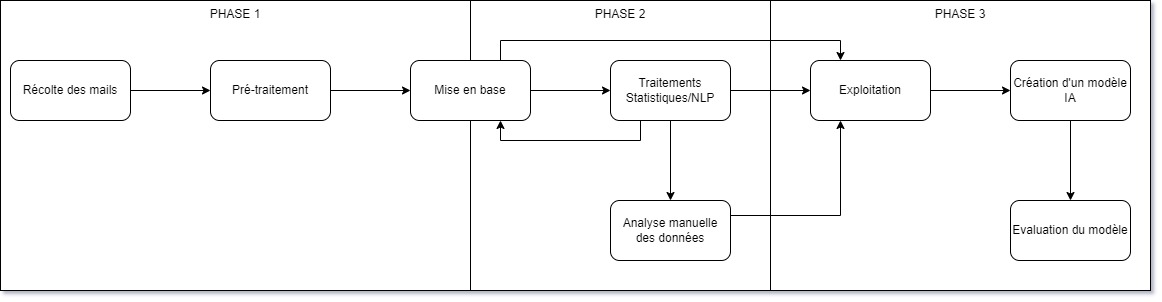
\includegraphics[width=\linewidth]{img/SchemaGeneral.jpg}
		\caption{Schéma des grandes étapes}
	\end{figure}
		 
\newpage

\section{Phase 1 : Récupération des données}
	La suite d'opération de cette phase vas permettre d'extraire un maximum d'information d'un email en essayant de ne dénaturer ni le fond ni la forme. Il pourra ensuite être stocké avec sa catégorie d'appartenance. Durant cette phase nous allons également initialiser les bases de données en créant les index (ES) et les tables (PSQL et SQLITE). 
	
	Ci-dessous le schéma général de cette phase.
	\begin{figure}[H]
		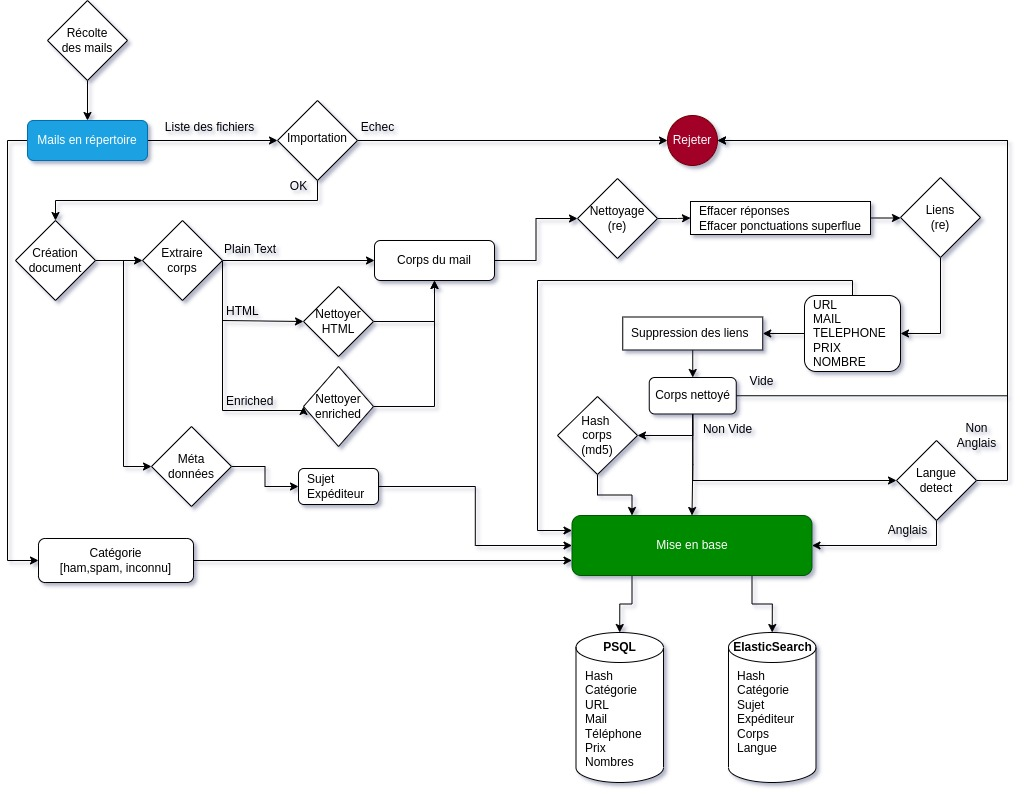
\includegraphics[width=\linewidth]{img/SchemaPhase1.jpg}
		\caption{Schéma des étapes de la phase 1}
	\end{figure}


	\subsection{Récolte des données}
		\paragraph{Recherche de dataset}
			Ma volonté initiale était de travailler sur des mails en français. Cependant, je n'ai pas trouvé de dataset dans cette langue. Je me suis donc retourné vers les dataset de mails en anglais. \\
			J'ai pu alors récupérer deux dataset:
			\begin{itemize}
				\item Enron company mails (voir: \ref{Enron_dataset})
				\item Dataset SpamAssassin (voir: \ref{SpamAssassin_dataset})
			\end{itemize}
			Les mails de SpamAssassin ont l'avantage d'être pré-trié, contrairement aux mails de la compagnie Enron. Ainsi le développement du moteur se fera uniquement avec les mails du SpamAssasin afin de pouvoir vérifier les résultats de l'analyse. 
		
		\paragraph{Téléchargement des données}
			Le téléchargement du dataset Enron est possible a partir du moment où l'on possède un compte sur la plateforme Kaggle. Le dataset SpamAssassin est ouvert, il suffit de télécharger les archives de chaque catégorie. \\
			
			La récolte des données a été réalisée à la main sans automatisation. 
			Les mails sont alors stockés dans plusieurs répertoires \emph{HAM} et \emph{SPAM} selon leur catégorie. \\
			
			Format:
			\begin{itemize}
				\item \emph{Enron} - 1 fichier CSV avec tous les mails
				\item \emph{SpamAssassin} - 1 fichier texte par mail
			\end{itemize}
	
	\subsection{Pré-traitement}
		Les étapes de pré-traitement regroupent toutes les étapes et actions réalisées avant la mise en base. 
		L'objectif de ces étapes est d'extraire le message en retirant les métadonnées du mail.
		Il va être possible d'effectuer certain traitement de nettoyage et de récupération d'informations primaires.
		
		Les manipulations de messages dans Python se font principalement à l'aide du module python natif \emph{email}. 
		
		\subsubsection{Importation}		
			La fonction \emph{email.message\_from\_binary\_file} permet de transformer un fichier mail en objet python manipulable :
			\begin{lstlisting}[title=Fonction d'importation des fichiers]
def import_from_file(chemin):
    try:
        with open(chemin, 'rb') as data:
            msg = message_from_binary_file(data, policy=policy.default)
            return msg
	
    except FileNotFoundError:
        print("Fichier : '{}' non trouve".format(chemin), file=sys.stderr)
        return None\end{lstlisting}
		
		
		\subsubsection{Extraction des corps des mails}
			Une fois le fichier importé au format \emph{EmailMessage}, il est possible d'en extraire le corps.
			
			Le corps du mail peut être composé de plusieurs parties qui ne sont pas forcément du texte. Les parties non textuelles ne sont pas conservée. 
					
		    	\begin{lstlisting}[title=Extraction du corps du mail]
def extract_body(msg):
    refused_charset = ['unknown-8bit', 'default', 'default_charset',
                       'gb2312_charset', 'chinesebig5', 'big5']
    body = ""

    if msg.is_multipart():
        for part in msg.walk():
            if not part.is_multipart():
                body += extract_body(part)
        return body

    if msg.get_content_maintype() != 'text':
        return ""

    if msg.get_content_charset() in refused_charset:
        return ""

    if msg.get_content_subtype() == 'plain':
        payload = msg.get_payload(decode=True)
        body += payload.decode(errors='ignore')

    if msg.get_content_subtype() == 'html':
        payload = msg.get_payload(decode=True)
        body += nettoyage.clear_html(payload.decode(errors='ignore'))

    if msg.get_content_subtype() == 'enriched':
        payload = msg.get_payload(decode=True)
        body += nettoyage.clear_enriched(payload.decode(errors='ignore'))

    return body \end{lstlisting}
	    		
		\subsubsection{Nettoyage}
			Le nettoyage du texte utilise principalement les expressions régulières pour retirer un maximum d'éléments indésirables dans le texte. J'utilise également 2 modules externes afin de traiter le code HTML et faire la détection des mails qui ne sont pas écrits en anglais.
			
			\paragraph{Par regex} J'utilise le module python \emph{re} pour réaliser les traitements suivants:
			
				\subparagraph{Suppression des réponses} Lorsque l'on répond à un mail, le texte du message précédent est conservé dans le corps du mail. Afin de permettre la distinction avec les mails précédant le caractère '>' est ajouté en début de ligne. Je retire toutes les lignes correspondant à des réponses afin de limiter les doublons.
				
					\begin{lstlisting}[title=Nettoyage des réponses]
def clear_reply(texte):
    pattern = re.compile('^>.*$', flags=re.MULTILINE)
    return re.sub(pattern, '', texte) \end{lstlisting}
					
				\subparagraph{Suppression des ponctuations} Afin de ne pas surcharger la base de données et pour se concentrer sur le texte, une grande partie des caractères de ponctuation seront retirés. L'idée est de se concentrer sur les ponctuations classiques (.,?!).

					\begin{lstlisting}[title=Nettoyage des ponctuations]				
def clear_ponctuation(texte):
    pattern_ponct = re.compile('[*#\\-_=:;<>\\[\\]"\'~)(|/$+}{@%&\\\]', flags=re.MULTILINE)
    return re.sub(pattern_ponct, ' ', texte) \end{lstlisting}

				% Suppression des balises pour les enriched text
				\subparagraph{Suppression des balises pour les enriched text} Certaines parties du corps de mail sont de type \emph{enriched text}. Les balises ne sont pas pertinente dans notre analyse et sont donc retirées.
						
					\begin{lstlisting}[title=Nettoyage des balises enriched text]
def clear_enriched(texte):
    pattern = re.compile('<.*>')
    return re.sub(pattern, '', texte) \end{lstlisting}
						
				% Modification des liens (URL, MAIL et TELEPHONE)
				\subparagraph{Suppression des liens} La présence de certaines informations comment les liens URL, les adresses mails et les numéros de téléphone ne peuvent pas être utilisés dans l'analyse textuelle. Cependant il peut être intéressant de conserver une trace de leur présence. Nous allons donc modifier ces liens qui seront comptabilisés avant d'être retirés du texte.
				
					\begin{lstlisting}[title=Nettoyage des liens]
def change_lien(texte, liens):
    pattern_mail = re.compile('[a-zA-Z0-9_.+-]+@[a-zA-Z0-9-]+\\.[a-zA-Z0-9-.]+')

    pattern_url1 = re.compile('(http|ftp|https)?:\/\/([\w\-_]+(?:(?:\.[\w\-_]+)+))'
                             '([\w\-\.,@?^=%&:/~\+#]*[\w\-\@?^=%&/~\+#])?', flags=re.MULTILINE)
    pattern_url2 = re.compile('(\\w+\\.)+\\w+', flags=re.MULTILINE)
    pattern_tel1 = re.compile('\\(\\d{3}\\)\\d+-\\d+')  # (359)1234-1000
    pattern_tel2 = re.compile('\\+\\d+([ .-]?\\d)+')    # +34 936 00 23 23

    temp, liens['MAIL'] = re.subn(pattern_mail, ' ', texte)

    temp, liens['URL'] = re.subn(pattern_url1, ' ', temp)
    temp, nb = re.subn(pattern_url2, ' ', temp)
    liens['URL'] += nb

    temp, liens['TEL'] = re.subn(pattern_tel1, ' ', temp)
    temp, nb = re.subn(pattern_tel2, ' ', temp)
    liens['TEL'] += nb

    return temp \end{lstlisting}
 
 
				% Modification des nombes (NOMBRE et PRIX)
				\subparagraph{Suppression des nombres} Comme pour les liens, les nombres sont comptabilisés et retirés. Je fais la distinction entre les nombres seuls et les nombres accompagnés de sigle monétaires. 
				
				\begin{verbatim}
monnaie = '€$£'
				\end{verbatim}
					\begin{lstlisting}[title=Nettoyage des nombres]
def change_nombres(texte, liens):
    pattern_prix1 = re.compile(f'[{monnaie}]( )?\\d+([.,]\\d+)? ', flags=re.MULTILINE)
    pattern_prix2 = re.compile(f' \\d+([.,]\\d+)?( )?[{monnaie}]', flags=re.MULTILINE)
    pattern_nb = re.compile('\\d+')

    temp, liens['PRIX'] = re.subn(pattern_prix1, ' ', texte)
    temp, nb = re.subn(pattern_prix2, ' ', temp)
    liens['PRIX'] += nb

    temp, liens['NOMBRE'] = re.subn(pattern_nb, ' ', temp)

    return temp \end{lstlisting}
 
 
			\paragraph{Par module}
				Lors du processus de nettoyage, j'utilise deux modules externes plus performants que ce que j'aurais pu faire simplement avec des expressions régulières. L'un me permet de nettoyer le code HTML, l'autre de détecter la langue du message. 
				
				% Suppression balise HTML avec BeautifulSoup
				\subparagraph{Suppression du code HTML} Certaines parties du corps du mail sont de type HTML. J'utilise le module \emph{BeautifulSoup} pour parser le code et récupérer le texte affiché. 
		
					\begin{lstlisting}[title=Nettoyage des nombres]		
from bs4 import BeautifulSoup

def clear_html(texte):
    brut = BeautifulSoup(texte, "lxml").text
    return brut \end{lstlisting}	
    		
				% Retrait des mails en langue non anglaise
				\subparagraph{Sélection des mails en anglais} Lors de mes tests, je me suis rendu compte que certains mails n'étaient pas en anglais. J'ai donc trouvé le module \emph{langdetect} qui permet de détecter le langage utilisé dans un texte en utilisant un modèle Naïve Bayes avec une précision de 99\% (voir \ref{langdetect}). \\
				Je conserve dans les données à mettre en base le langage détecté avec l'idée de pouvoir traité plusieurs langues dans le futur.\\
				
				La détection de la langue est réalisée juste avant la mise en base dans l'index ElasticSearch.
				
				\begin{lstlisting}[title=Création d'un document]	
import langdetect

def create_document(mail, categorie):
    corp = mail_load.extract_body(mail)
    corp, liens = nettoyage.clear_texte_init(corp)
    sujet, expediteur = mail_load.extract_meta(mail)

    if not corp:
        return None

    try:
        lang = langdetect.detect(corp)
    except langdetect.lang_detect_exception.LangDetectException:
        return None

    if lang != 'en':
        return None

    if categorie.lower() not in ['spam', 'ham']:
        categorie = 'inconnu'

    doc = {
        'hash': hashlib.md5(corp.encode()).hexdigest(),
        'categorie': categorie.lower(),
        'sujet': sujet,
        'expediteur': expediteur,
        'message': corp,
        'langue': lang,
        'liens': liens
    }
    return doc \end{lstlisting}
 
 
			\paragraph{Exemple de traitement}
				Les sections suivantes présentent des exemples de traitement de la phase 1.
				
				\begin{lstlisting}[title=Traitement initial]
message = '''
Message dedicated to be a sample to show how the process is clearing the text.

Begin reply :
> He once said
>>> that it would be great
End of reply.

Substitutions :
spamassassin-talk@example.sourceforge.net
https://www.inphonic.com/r.asp?r=sourceforge1&refcode1=vs3390
hello.foo.bar
between $ 25 and 25,21 $

A number is : 2588,8 588
Phone type a : (359)1234-1000
Phone type b : +34 936 00 23 23
Ponctuation : ----## ..
~ ~~~~~
'''
text, liens = clear_texte_init(message)
print(liens)
print(text) 
				\end{lstlisting}

				Résultat traitement initial :
				\begin{verbatim}
{'URL': 2, 'MAIL': 1, 'TEL': 2, 'NOMBRE': 3, 'PRIX': 2}

Message dedicated to be a sample to show how the process is clearing the text.

Begin reply 


End of reply.

Substitutions 



between and

A number is  , 
Phone type a  
Phone type b  
Ponctuation   ..
				\end{verbatim}
				
				\begin{lstlisting}[title=Traitement HTML]
message_html = '''
<!DOCTYPE html PUBLIC "-//W3C//DTD HTML 4.01 Transitional//EN">
<html>
<head>
  <title>Foobar</title>
</head>
<body>
I actually thought of this kind of active chat at AOL 
bringing up ads based on what was being discussed and 
other features
  <pre wrap="">On 10/2/02 12:00 PM, "Mr. FoRK" 
  <a class="moz-txt-link-rfc2396E"href="mailto:fork_
  list@hotmail.com">&lt;fork_list@hotmail.com&gt;</a> 
  wrote: Hello There, General Kenobi !?
<br>
</body>
</html>
'''
print(clear_html(message_html))
				\end{lstlisting}
				Résultat traitement HTML :
				\begin{verbatim}

Foobar


I actually thought of this kind of active chat at AOL 
bringing up ads based on what was being discussed and 
other features
  On 10/2/02 12:00 PM, "Mr. FoRK" 
  <fork_list@hotmail.com> 
  wrote: Hello There, General Kenobi !?


				\end{verbatim}

				\begin{lstlisting}[title=Traitement enriched text]
message_enriched = '''
<smaller>I'd like to swap with someone also using Simple DNS to take
advantage of the trusted zone file transfer option.</smaller>
'''
print(clear_enriched(message_enriched))
				\end{lstlisting}
				Résultat traitement enriched text :
				\begin{verbatim}
I'd like to swap with someone also using Simple DNS to take
advantage of the trusted zone file transfer option.
				\end{verbatim}


		\subsubsection{Mise en base}
			Cette section détaille les éléments relatifs à la mise en base des informations récoltées. Dans ce projet, j'utilise 2 moteurs de bases de données pour stocker les données des mails. 
			\begin{enumerate}
				\item un index ElasticSearch pour faire le stockage des données textuelles
				\item une base PostgreSQL pour le stockage des données numériques
			\end{enumerate}
				 
			J'utilise des conteneurs \emph{docker} pour héberger les services de bases de données. 
			L'utilisation des conteneurs me permet de partager plus facilement mes configurations et limite les erreurs d'installations.\\
			
			% Déroulé de la mise en base
			Pour chaque mail récolté le programme de la phase 1 va générer un \emph{document} avec les informations suivantes :
				\begin{itemize}
					\item hash - signature md5 du texte nettoyé 
					\item catégorie - Ham, Spam ou Inconnu
					\item sujet - correspond à l'objet du mail
					\item expéditeur - adresse mail
					\item corps - corps du mail nettoyé
					\item langue - la langue détectée du mail (en)
					\item liens - données non textuelles extraites du corps :
						\begin{itemize}
							\item[•] URL - liens URL
							\item[•] Mail - adresses mail
							\item[•] Téléphone - numéros de téléphone
							\item[•] Prix - nombres avec un symbole de devise
							\item[•] Nombres
						\end{itemize}
				\end{itemize}
				
				Chaque document va générer une entrée dans la base ElasticSearch et une entrée dans la base PostgreSQL. 
				
				\begin{lstlisting}[title=Création d'un document]
def create_document(mail, categorie):
    corp = mail_load.extract_body(mail)
    corp, liens = nettoyage.clear_texte_init(corp)
    sujet, expediteur = mail_load.extract_meta(mail)

    if not corp:
        return None

    try:
        lang = langdetect.detect(corp)
    except langdetect.lang_detect_exception.LangDetectException:
        return None

    if lang != 'en':
        return None

    if categorie.lower() not in ['spam', 'ham']:
        categorie = 'inconnu'

    doc = {
        'hash': hashlib.md5(corp.encode()).hexdigest(),
        'categorie': categorie.lower(),
        'sujet': sujet,
        'expediteur': expediteur,
        'message': corp,
        'langue': lang,
        'liens': liens
    }
    return doc
				\end{lstlisting}
			
			Ci-dessous le schéma des bases de données avec les relations entre elles.			
			\begin{figure}[H]
				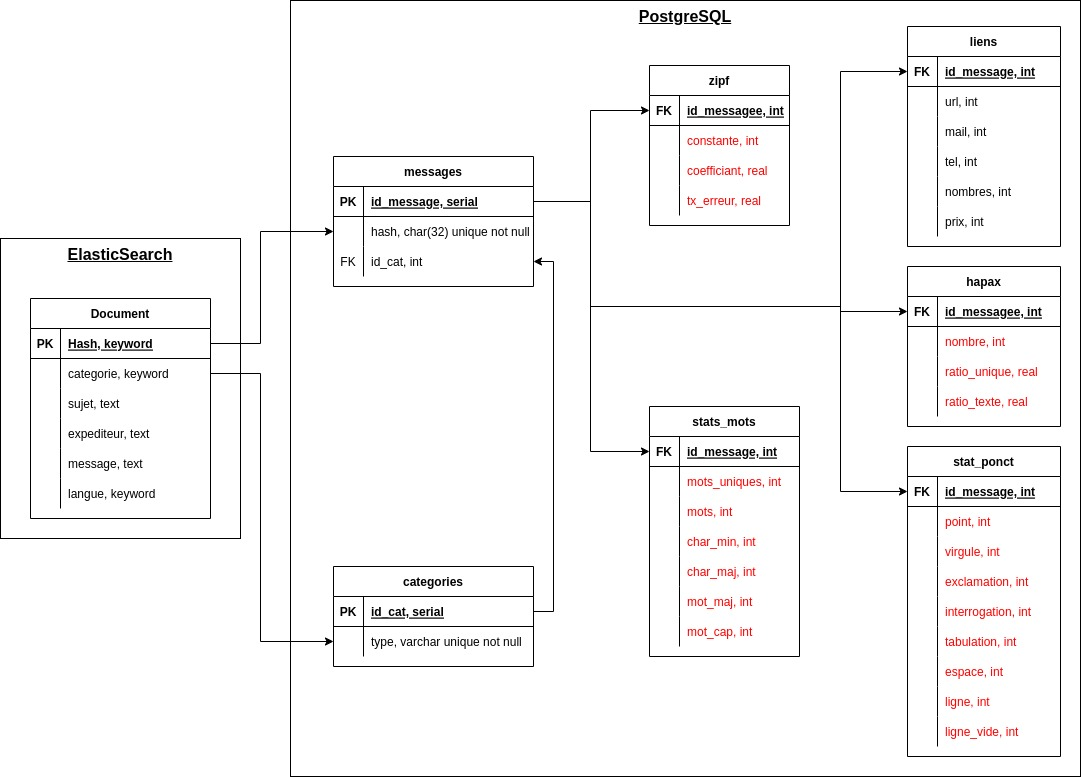
\includegraphics[width=\linewidth]{img/SchemaBdd.jpg}
				\caption{Schéma des bases de données de l'application}
			\end{figure}
			Le \emph{hash} calculé lors de la phase de traitement est l'identifiant unique du mail dans toutes les bases. La catégorie du mail est également présente dans les deux bases. 
			Les champs en rouge sont des caractéristiques qui ne sont pas calculées lors de la phase 1.
		
			\paragraph{Stockage des données: ElasticSearch}
				ElasticSearch est un moteur de base de données NoSQL. Il intègre un moteur d'indexation des documents est assez performant pour stocker des données textuelles de taille aléatoire. 
				Il est cependant assez compliqué de modifier le schéma d'un index une fois qu'il a été créé. Pour ces raisons, j'utilise cette technique pour ne stocker que les données textuelles après nettoyage car elles n'ont plus vocation à être modifiées. \\
				
				Les corps de mail mis en base seront récupérés ultérieurement pour réaliser les opérations d'analyse. Les résultats seront stockés dans la base PostgreSQL, plus souple. \\
				
				Ci-dessous les fonctions principales pour l'ajout d'un document dans la base ES.
				\begin{lstlisting}[title=Fonctions basique pour la liaison ElasticSearch]
def es_connect(server, creds, crt):
    """ Connexion au serveur ElasticSearch """
    client = Elasticsearch(server, api_key=creds, ca_certs=crt)

    try:
        client.search()
        client.indices.get(index="*")
        return client

    except (exceptions.ConnectionError, AuthenticationException, AuthorizationException) as err:
        print("ES:conn - Informations client ElasticSearch :\n\t", err)
        client.close()
        return None
        

def es_index_doc(es_cli, index, doc):
    """ Index un document dans la base ES """
    id_doc = doc['hash']

    if es_document_exists(es_cli, index, id_doc):
        return 1

    es_cli.index(index=index, document=doc)
    es_cli.indices.refresh(index=index)
    return 


def es_document_exists(es_cli, index, hash):
    """ Regader dans l'index si le hash du document est deja present """
    try:
        resp = es_cli.search(index=index, query={"match": {"hash": hash}})
    except elasticsearch.NotFoundError as err:
        print("Error : hash", err, file=sys.stderr)
        return None

    return True if resp['hits']['total']['value'] == 1 else False
				\end{lstlisting}
				
				Le déploiement et les configurations de la base ElasticSearch sont disponibles dans l'annexe \ref{ES}.
				
				
			\paragraph{Stockage des premières informations statistiques: PostgreSQL} Pour le stockage des données statiques et d'analyse, j'ai décidé de m'orienter vers le système de gestion de base de données PostgreSQL. Une base de données relationnelle est plus flexible qu'un index ElasticSearch pour l'ajout de nouvelles caractéristiques. \\
			
				Durant la phase 1, j'utilise que 3 tables :
				\begin{itemize}
					\item messages - liste des mails avec le hash permettant de faire le lien avec l'index ES
					\item categorie - liste des catégories de mails
					\item liens - comptabilise le nombre d'occurrences par type de lien ou nombre
				\end{itemize}
				
				Cette base a pour but de stocker les données formatées pour l'analyse, l'exploitation et l’entraînement du modèle.
			
				\begin{lstlisting}[title=Fonctions basiques pour la liaison PostgreSQL]
def connect_db(database, user, passwd, host, port):
    """ Connexion a la base de donnees Postgres """
    try:
        client_psql = psycopg2.connect(database=database, user=user, password=passwd, host=host, port=port)
    except psycopg2.Error as e:
        print("Erreur de connexion : \n{}".format(e), file=sys.stderr)
        return None

    client_psql.autocommit = True
    return client_psql
    
    
def insert_data(client_psql, table, data):
    """
    Insere les donnees d'un dictionnaire dans une table de la base de donnees PSQL
    Les cles du dictionnaire doivent correspondre aux colonnes de la table.
    """
    cols = ','.join([str(c) for c in data.keys()])
    vals = ','.join([str(v) if (type(v) != str) else f"'{v}'" for v in data.values()])
    query = f"INSERT INTO {table}({cols}) VALUES ({vals})"

    exec_query(client_psql, query)


def get_data(client_psql, table, champs, clause=None):
    """ Recupere les donnees de la base. """
    query = f"SELECT {','.join(champs)} FROM {table}"
    if clause:
        query += f" WHERE {clause}"

    result = exec_query(client_psql, query)
    return [dict(zip(champs, ligne)) for ligne in result]
    
    
def insert_document_init(client_psql, data, id_cat):
    """ Insere un nouveau document dans la base PSQL. """
    insert_data(client_psql, 'messages', {'hash': data['hash'], 'id_cat': id_cat})
    id_message = get_data(client_psql, 'messages', ['id_message'], f"hash LIKE '{data['hash']}'")[0]['id_message']

    liens = data['liens']
    liens.update({'id_message': id_message})
    insert_data(client_psql, 'liens', liens)   
    
def exec_query(client_psql, query):
    """ Execute une query dans la base PSQL """
    cursor = client_psql.cursor()

    try:
        cursor.execute(query)
        if query.upper().find("SELECT", 0, 6) >= 0:
            return cursor.fetchall()
        return []
    except psycopg2.Error as e:
        print("Erreur d'execution de la requete : {}".format(e), file=sys.stderr)
        print("requete : {}".format(query), file=sys.stderr)
        return []
				\end{lstlisting}
				
				Le déploiement et les configurations de la base PostgreSQL sont disponibles dans l'annexe \ref{PSQL}.
			
			
			\paragraph{Stockage des données statistiques du traitement: SQLite}
				Les données présentent dans cette base permettent de suivre l'évolution de certaines métriques lors des différentes étapes du nettoyage. 
				A chaque grandes étapes de la phase 1 (Importation, Nettoyage, Mise en base), je calcule pour les HAM, SPAM et (HAM+SPAM) les éléments suivants :
				\begin{itemize}
					\item mails - nombre de mails
					\item mots - nombre de mots dans tout le corpus
					\item mots\_uniques - nombre de mots uniques dans tout le corpus
				\end{itemize}
				
				Ces données me permettent d'estimer la quantité de données nettoyées durant cette phase.
				
				\begin{figure}[H]
					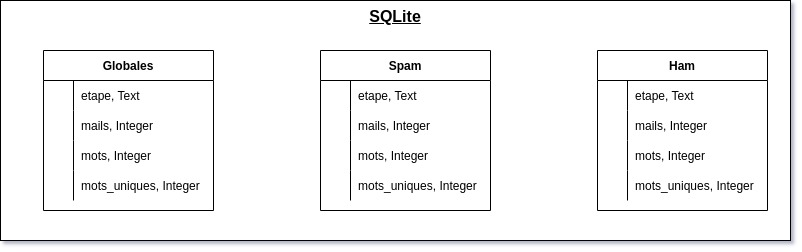
\includegraphics[width=\linewidth]{img/Schemasqlite.jpg}
					\caption{Schéma de la base de données pour lors du traitement}
				\end{figure}
							
			
	
	\subsection{Données de la phase 1}
		Sortie du programme : main\_collecte.py
		\begin{verbatim}
=== Vérification des conteneurs Docker ===
* Conteneur 'docker-es01-1'... OK
* Conteneur 'docker-kibana-1'... OK
* Conteneur 'docker_pgadmin_1'... OK
* Conteneur 'docker_pgdb_1'... OK
=== Phase 1 : collecte & mise en base ===
== Création de la base SQLITE
SQLITE table globales : CREATED
SQLITE table spam : CREATED
SQLITE table ham : CREATED
== Recolte ==
-- Création de la liste des fichiers... OK
--- Process de statistiques après la récole
-- Stats - étape : Récolte spam... OK                                                                                                                                                                                                         
-- Stats - étape : Récolte ham... OK                                                                                                                                                                                                          
--- Sauvegarde des stats de l'étape: recolte... OK
Données stats de l'étape: recolte:
	HAM,  mails: 4153 	mots: 1863674	 mots uniques: 178812
	SPAM,  mails: 1898 	mots: 918256	 mots uniques: 129601
	GLOBALES,  mails: 6051 	mots: 2781930	 mots uniques: 287637
== Création document ==
-- Importation - Création spam... OK                                                                                                                                                                                                          
-- Importation - Création ham... OK                                                                                                                                                                                                           
--- Process de statistiques après la création de document
-- Stats - étape : création documents spam... OK                                                                                                                                                                                              
-- Stats - étape : création documents ham... OK                                                                                                                                                                                               
--- Sauvegarde des stats de l'étape: creation document... OK
Données stats de l'étape: creation document:
	HAM,  mails: 4124 	mots: 844151	 mots uniques: 73725
	SPAM,  mails: 1784 	mots: 584012	 mots uniques: 40099
	GLOBALES,  mails: 5908 	mots: 1428163	 mots uniques: 97235
== Mise en base des documents ==
-- Création de l'index ElasticSearch... OK
-- Création de la base PostgreSQL
User 'data' déjà existant
-- Création des tables PostgreSQL... OK
-- Mise en base ES & PSQL des spam... OK (256 doublons)                                                                                                                                                                                       
-- Mise en base ES & PSQL des ham... OK (78 doublons)                                                                                                                                                                                         
-- Récupération des spam... OK
-- Récupération des ham... OK
--- Process de statistiques après la mise en base
-- Stats - étape : Mise en base spam... OK                                                                                                                                                                                                    
-- Stats - étape : Mise en base ham... OK                                                                                                                                                                                                     
--- Sauvegarde des stats de l'étape: mise en base... OK
Données stats de l'étape: mise en base:
	HAM,  mails: 4046 	mots: 839368	 mots uniques: 73725
	SPAM,  mails: 1528 	mots: 529121	 mots uniques: 40099
	GLOBALES,  mails: 5574 	mots: 1368489	 mots uniques: 97235
== FIN ==

		\end{verbatim}
		
		\paragraph{Évolution lors du traitement}
			Les données recueillis pendant le traitement permettent de constater les comportements suivants:
			\begin{itemize}
				\item La diminution des documents spam est plus importante que celle des ham 
				\item Le nombre de mots uniques ne diminue plus après la création de document
				\item La diminution du nombre de mots est plus importante dans les ham que dans les spam. 
				\item le nombre de mot uniques est plus important dans les ham que dans les spam
			\end{itemize}
			
			\begin{figure}[H]
				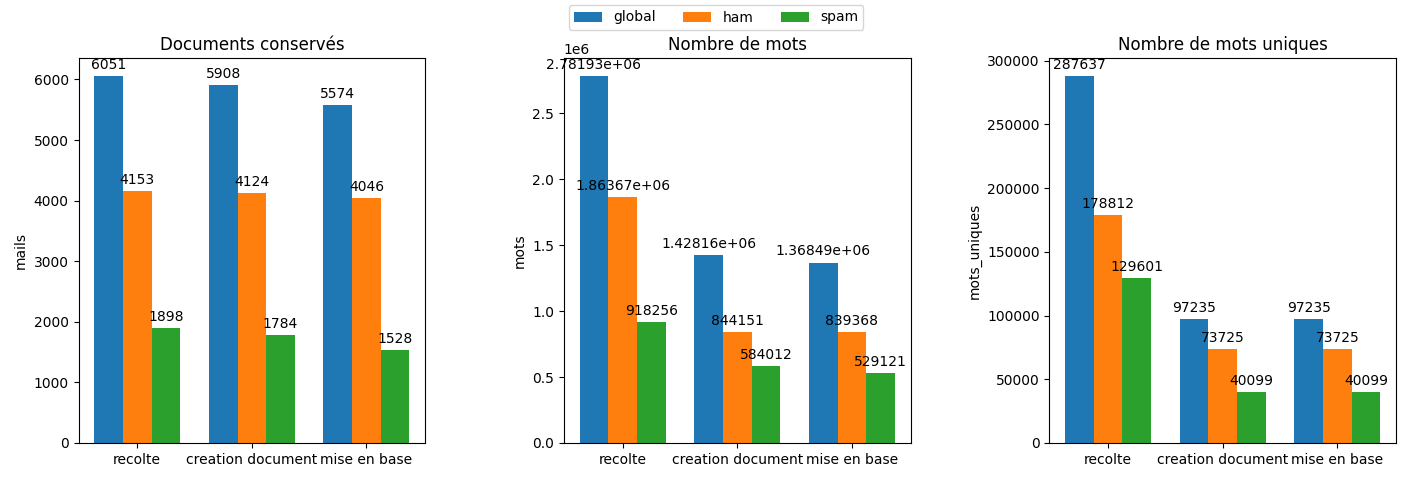
\includegraphics[width=\linewidth]{img/Statsrecolte.png}
				\caption{Évolution des principaux marqueurs lors du traitement}
			\end{figure}
		
			\subparagraph{Conclusion de la récolte}
				A l'issue de la phase de récolte, on remarque qu'il y a un nombre plus important de document en double dans la catégorie \emph{spam}.				
				Il y a également une réduction importante du nombre de mots ainsi que du nombre de mots uniques dans les \emph{ham}. Cette réduction peut s'expliquer par le nettoyage du corps des mails :
				\begin{itemize}
					\item Retrait des réponses
					\item Retrait de certaines ponctuations
					\item Suppression des balises HTML et enriched text
					\item Retrait des liens, et nombres
				\end{itemize}
				
				Enfin on peut voir que les \emph{ham} utilisent plus de mots uniques que les \emph{spam}. Il est donc possible que le vocabulaire des \emph{spam} soit plus restreint. 
			
				
		\paragraph{Premières données statistiques}
			Les documents conservés à l'issue de cette phase de récupération se constitue à $72,6\%$ de Ham et à $27.4\%$ de Spam.
			
			\begin{figure}[H]
				\centering
				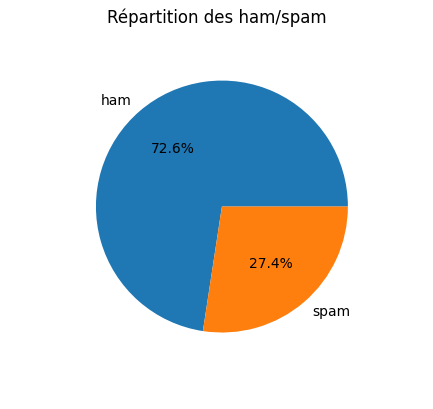
\includegraphics[scale=1]{img/hamSpam.png}
				\caption{Répartition des ham/spam dans le dataset}
			\end{figure}
			
			Grâce aux informations et des pré-traitements réalisés lors de cette première phase, il est possible de présenter quelques données statistiques. Notamment sur la présence et l'utilisation de liens (url, mail, téléphonique) et des données numériques (nombres et prix).\\

			\begin{table}[H]
					\centering
					\captionof{table}{Statistiques sur les liens} \label{tab:p1liens}
					\begin{tabular}{|l|c|c|c|c|c|c|c|c|c|}
						\hline
						 	& \multicolumn{3}{|c|}{url} & \multicolumn{3}{|c|}{mail} & \multicolumn{3}{|c|}{tel}\\
						 	& Globale & Ham & Spam & Globale & Ham & Spam & Globale & Ham & Spam \\
						\hline
						moyenne    & 5.47 & 5.54 & 5.26 & 1.16 & 1.21 & 1.01 & 0.16 & 0.20 & 0.64 \\
						\hline
						écart-type & 49.74 & 57.77 & 13.71    & 2.50 & 1.72 & 3.88     & 1.06 & 0.63 & 1.73 \\
						\hline
						minimum    & \multicolumn{3}{|c|}{0} & \multicolumn{3}{|c|}{0} & \multicolumn{3}{|c|}{0} \\
						\hline
						25\%       & \multicolumn{3}{|c|}{1}     & \multicolumn{3}{|c|}{0}    & \multicolumn{3}{|c|}{0} \\
						\hline
						médiane    & 2 & 2 & 3     & 1 & 1 & 0   & \multicolumn{3}{|c|}{0} \\
						\hline
						75\%       & 4 & 4 & 5    & 2 & 2 & 1    & \multicolumn{3}{|c|}{0} \\
						\hline
						maximum    & 3557 & 3557 & 295  & 69 & 34 & 69  & 67 & 25 & 67 \\
						\hline
					\end{tabular}
				\end{table}
				
				A partir des données des liens présentées dans le tableau ci-dessus il est possible d'émettre les hypothèses suivantes.\\
				On trouve en moyenne environ 5 url dans les deux types de mails. Cependant la dispersion est notablement plus faible pour les spams. On voit également que $75\%$ des spam contiennent 5 liens ou moins. \\
				La présence d'adresses mail est assez marginale environ une adresse mail par corps de texte. L'écart-type est plus faible dans les ham. On voit également que $75\%$ des ham contiennent deux adresse mails ou moins contre 1 pour les spam.\\
				Enfin la présence de numéro de téléphone est quasiment nulle pour les deux catégories. 
				
				\begin{table}[H]
					\centering
					\captionof{table}{Statistiques sur les données numériques} \label{tab:p1nb}
					\begin{tabular}{|l|c|c|c|c|c|c|}
						\hline
						 	& \multicolumn{3}{|c|}{nombre} & \multicolumn{3}{|c|}{prix} \\
						 	& Globale & Ham & Spam & Globale & Ham & Spam \\
						\hline
						moyenne    & 15.14 & 9.38 & 30.38 & 0.28 & 0.08 & 0.81\\
						\hline
						écart-type & 219.16 & 49.35 & 410.53    & 1.54 & 0.66 & 2.66 \\
						\hline
						minimum    & \multicolumn{3}{|c|}{0} & \multicolumn{3}{|c|}{0} \\
						\hline
						25\%       & 1 & 1 & 2      & \multicolumn{3}{|c|}{0} \\
						\hline
						médiane    & 5 & 5 & 7     & \multicolumn{3}{|c|}{0} \\
						\hline
						75\%       & 9 & 8 & 14     & \multicolumn{3}{|c|}{0} \\
						\hline
						maximum    & 15801 & 2794 & 15801  & 29 & 17 & 29 \\
						\hline
					\end{tabular}
				\end{table}
				
				Les données numériques du dataset montrent les hypothèses suivantes.\\
				Les nombres simples semblent être les données les plus présentes dans le corps du mail, environ $15$ en moyenne par mail, cependant la dispersion est élevée. Cela étant $75\%$ des spam ont $14$ nombres ou moins contre $8$ ou moins pour les ham.\\
				Enfin la présence de prix est assez marginale par rapport aux nombres. Il y a cependant en moyenne 10 fois plus de prix dans les spam que les ham.\\
			
			\begin{figure}[H]
				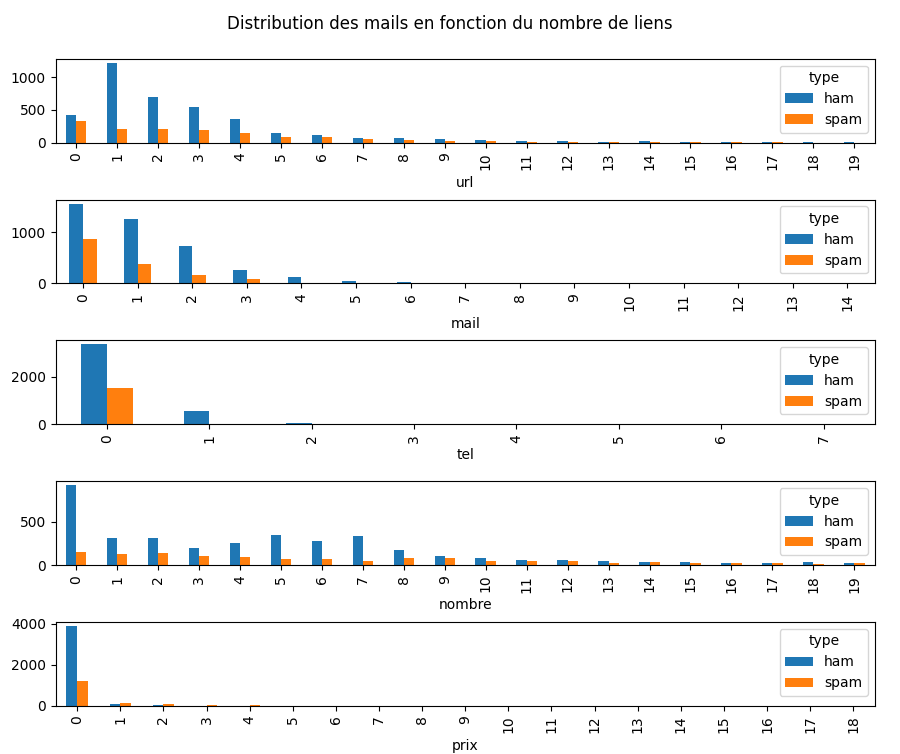
\includegraphics[width=\linewidth]{img/P1feat.png}
				\caption{Distribution du nombre de liens selon la catégorie du mail}
			\end{figure}
			
			
			Au vu des analyses précédents, on peut dire qu'il est statistiquement plus probable de trouver dans les spam plus de liens url, de nombre et de prix que dans les ham. La présence d'adresse mail est plus probable dans les ham. Il est enfin possible d'exclure la présence de numéro de téléphone qui est trop marginale.\\
			
			Les codes sources de cette partie sont disponibles dans le fichier \emph{./analyse/analyse\_p1.py} ou dans la section \ref{subsec:analp1}
			
			
			
 
	
\newpage
\section{Phase 2: Traitement des données}
	Les opérations de cette phase ont pour but d'extraire les caractéristiques des textes collectés à la phase précédente. 
	Puis, Nous allons rechercher des informations numériques sur la forme des messages (nombre de mots, de ponctuations,...).  
	Enfin, nous appliqueront des techniques de traitement du langage naturel pour travailler sur le fond des corps de mail. 
	
	\subsection{Génération des données statistiques}
		Nous verrons ici le code utilisé pour récupérer ou générer les données des caractéristiques pour chaque message ainsi que la distribution de Zipf de manière globale.
		\begin{figure}[H]
			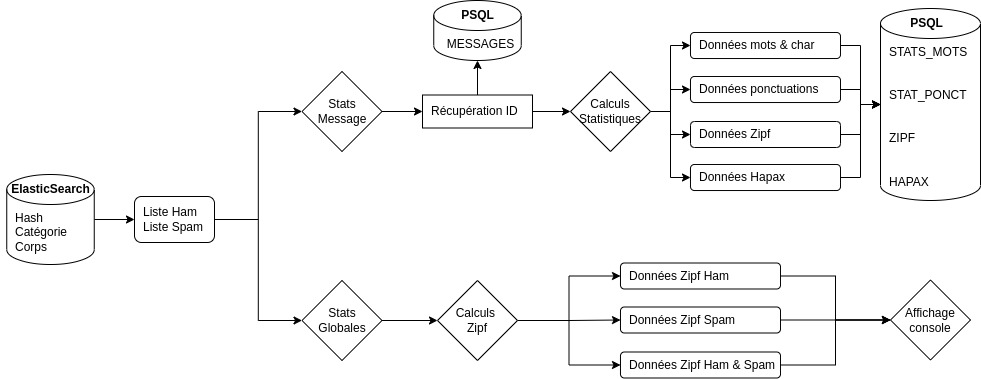
\includegraphics[width=\linewidth]{img/SchemaPhase2.jpg}
			\caption{Schéma des étapes de récupération des données}
		\end{figure}
		
		Les mails sont récupérés dans la base ElasticSearch. Les Ham et les Spam sont séparés dans deux listes distinctes.
		\begin{lstlisting}[title=Récupération des messages dans la base ES]
def recup_mails(es_index):
    es_cli = elastic_cmd.es_connect(es_secrets.serveur, (es_secrets.apiid, es_secrets.apikey), es_secrets.ca_cert)
    data = {}
    for cat in ['spam', 'ham']:
        print("-- Recuperation des {}...".format(cat), end=' ')
        data[cat] = {entry.get('_source').get('hash'): entry.get('_source').get('message') for entry in elastic_cmd.es_get_all(es_cli, es_index, sort={'hash': 'asc'},query={'match': {'categorie': cat}})}
        print('OK')
    return data		
		\end{lstlisting}
		
		Chaque message va ensuite passer par une série de traitement pour générer les données des caractéristiques avant d'être mise en base dans Postgresql. 
		
		\begin{lstlisting}[title=Pipeline pour chaque message]
def stats_pipe_message(hash_message, message, psql_cli):
    resp = psql_cmd.get_data(psql_cli, 'messages', ['id_message'], f"hash LIKE '{hash_message}'")
    if not resp:
        print(f"No id_message found for {hash_message}", file=sys.stderr)
        return
    id_mess = resp[0].get('id_message')

    for table, stat_func in {'stat_ponct': stats_ponct,
                             'stats_mots': stats_mot,
                             'zipf': stats_zipf,
                             'hapax': stats_hapax}.items():
        resp = psql_cmd.get_data(psql_cli, table, ['id_message'], f"id_message={id_mess}")
        if resp:
            continue
        psql_cmd.insert_data(psql_cli, table, stat_func(id_mess, message)
        
def stats_ponct(id_text, texte):
    return {
        "id_message": id_text,
        "point": texte.count('.'),
        "virgule": texte.count(','),
        "exclamation": texte.count('!'),
        "interrogation": texte.count('?'),
        "tabulation": texte.count('\t'),
        "espace": texte.count(' '),
        "ligne": texte.count('\n') + 1,
        "ligne_vide": len(re.findall(r'^\s*$', texte, re.MULTILINE))
    }


def stats_mot(id_text, texte):
    tokens = re.findall(r'\w+', texte, re.MULTILINE).
    return {
        'id_message': id_text,
        'char_min': len(re.findall(r'[a-z]', texte, re.MULTILINE)),
        'char_maj': len(re.findall(r'[A-Z]', texte, re.MULTILINE)),
        'mots': len(tokens),
        'mots_uniques': len(set(tokens)),
        'mot_maj': sum(mot.isupper() for mot in tokens),
        'mot_cap': sum(bool(re.match(r'[A-Z][a-z]+', mot)) for mot in tokens)
    }


def stats_zipf(id_text, texte):
    tokens = re.findall(r'\w+', texte, re.MULTILINE)
    data = stats.zipf_process(tokens)
    data['id_message'] = id_text
    data['constante'] = data.pop('const_moy')
    data['coefficient'] = data.pop('coef_min')
    data['tx_erreur'] = data.pop('cout_min')
    return data


def stats_hapax(id_text, texte):
    tokens = re.findall(r'\w+', texte, re.MULTILINE)
    data = stats.hapax(tokens)
    data['id_message'] = id_text
    data['nombre'] = data.pop('nombres')
    data['ratio_unique'] = data.pop('ratio_mots_uniques')
    return data
		\end{lstlisting}
		
	J'ai également réaliser les calculs de la distribution de Zipf sur l'ensemble du corpus ainsi que sur le regroupement des Ham et des Spam pour voir si des différences majeures pouvaient être mises en lumière. Les résultats de cette recherche sont affiché directement dans la console.
		
		\begin{lstlisting}[title=Pipeline pour les données globales]
def stats_pipe_globale(data):
    ls_ham = [mess for mess in data['ham'].values()]
    ls_spam = [mess for mess in data['spam'].values()]
    tokens = []
    for mess in ls_ham + ls_spam:
        tokens += re.findall(r'\w+', mess, re.MULTILINE)
    data = stats.zipf_process(tokens, True)
    print("Donnees Zipf ham+spam:", data)
    data = stats.hapax(tokens)
    print("Donnees Hapax ham+spam:", data)

    tokens = []
    for mess in ls_ham:
        tokens += re.findall(r'\w+', mess, re.MULTILINE)
    data = stats.zipf_process(tokens, True)
    print("Donnees Zipf ham:", data)
    data = stats.hapax(tokens)
    print("Donnees Hapax ham:", data)

    tokens = []
    for mess in ls_spam:
        tokens += re.findall(r'\w+', mess, re.MULTILINE)
    data = stats.zipf_process(tokens, True)
    print("Donnees Zipf spam:", data)
    data = stats.hapax(tokens)
    print("Donnees Hapax spam:", data
		\end{lstlisting}
	
	Les fonctions pour les instructions pour la distribution de Zipf sont donnés dans l'annexe \ref{sec:devZipf}.
		
	\subsection{Sortie de la partie 2: Stats d'exploitation}
		\begin{verbatim}
=== Phase 2 : Stats Exploitation ===
-- Récupération des spam... OK
-- Récupération des ham... OK
-- Récupération des statistiques par message
Stats Spam... OK
Stats Ham... OK
-- Récupérations des statistiques globales
Données Zipf ham+spam: {'const_moy': 73746.97464716957, 'cout_min': 6.37798252533617, 
	'coef_min': 0.93}
Données Hapax ham+spam: {'nombres': 33666, 'ratio_mots_uniques': 0.47656526478207323, 
	'ratio_texte': 0.024792183385275213}
Données Zipf ham: {'const_moy': 52712.404742906976, 'cout_min': 4.193202011347324, 
	'coef_min': 0.93}
Données Hapax ham: {'nombres': 26231, 'ratio_mots_uniques': 0.48674175650850793, 
	'ratio_texte': 0.03150367568904908}
Données Zipf spam: {'const_moy': 35485.13912209956, 'cout_min': 4.848725944493132, 
	'coef_min': 0.93}
Données Hapax spam: {'nombres': 12396, 'ratio_mots_uniques': 0.4097309446684736, 
	'ratio_texte': 0.023598168648092978}
		\end{verbatim}
	
	\subsection{Analyses statistiques}
		Dans cette partie nous nous intéressons aux données statistiques des caractéristiques récupérées lors de la phase précédente. 
		Nous verrons dans un premier temps les données des mots:
		\begin{itemize}
			\item nombre de mots
			\item nombre de mots uniques
			\item nombre de caractère en minuscule
			\item nombre de caractère en majuscule
			\item nombre de mots écrits complètement en majuscule
			\item nombre de mots écrits complètement avec la première lettre en capitale
		\end{itemize}
		A cela nous ajouterons une recherche de caractéristique sur les données de ponctuation:
		\begin{itemize}
			\item nombre de points '.'
			\item nombre de virgules ','
			\item nombre de points d'exclamation
			\item nombre de points d'interrogation
			\item nombre de tabulations
			\item nombre d'espaces
			\item nombre de lignes totales
			\item nombre de lignes vides
		\end{itemize}
		Enfin nous appliquerons les méthodes de distribution de Zipf sur chaque message\footnote{J'ai conscience que cette distribution est plus pertinente quand le corpus est grand}. Nous récupérerons alors les données suivantes
		\begin{itemize}
			\item constante estimée
			\item coefficient estimées
			\item taux d'erreur absolu moyen entre les fréquences réelles et théoriques de chaque mot
			\item nombre de mots n'apparaissant qu'une seule fois dans le texte (hapax)
			\item nombre d'hapax par rapport au vocabulaire du texte
			\item nombre d'hapax par rapport au total des mots du texte
		\end{itemize}
		
		\paragraph{Statistiques des mots et caractères}
			\begin{table}[htbp]
				\centering
				\captionof{table}{Statistiques sur les données des mots} \label{tab:smots}
				\resizebox{\columnwidth}{!}{\begin{tabular}{|l|c|c|c|c|c|c|c|c|c|c|c|c|}
					\hline
								& \multicolumn{3}{|c|}{nombre de mots} & \multicolumn{3}{|c|}{mots uniques} & \multicolumn{3}{|c|}{mots capitalisés} & \multicolumn{3}{|c|}{mots majuscules} \\
								& Global		& Ham 	& Spam 	& Global		& Ham	& Spam	& Global		& Ham	& Spam	& Global		& Ham	& Spam	\\
					\hline
					moyenne		& 243		& 205	& 343	& 130		& 116	& 167	& 41			& 34		& 59		& 14			& 8		& 29		\\
					\hline
					écart-type	& 586		& 531	& 701	& 187		& 180	& 198	& 114		& 111	& 119	& 49			& 39		& 66		\\
					\hline
					minimum		& 1			& 3		& 1		& 1			& 3		& 1		& 0			& 0		& 0		& 0			& 0		& 0		\\
					\hline
					25\%			& 53			& 44		& 94		& 46			& 39		& 73		& 9			& 8		& 15		& 2			& 2		& 3		\\
					\hline
					médiane		& 105		& 85		& 161	& 80			& 68		& 110	& 17			& 14		& 32		& 4			& 3		& 10		\\
					\hline
					75\%			& 215		& 174	& 326	& 139		& 120	& 191	& 35			& 25		& 60		& 10			& 7		& 24		\\
					\hline
					maximum		& 14127		& 14127	& 11274	& 4322		& 4322	& 2479	& 4656		& 4656	& 2192	& 1969		& 1969	& 763	\\
					\hline
				\end{tabular}}
			\end{table}
			Le tableau \ref{tab:smots}, sur les données des mots, montre que les Spam ont généralement plus de mots, 343 contre 205 en moyenne pour les Hams. Cela est également vrai pour les mots uniques par messages, les spams en contiennent globalement plus. Concernant la forme des mots, on voit que les mots avec majuscules sont plus souvent utilisés dans les Spam. Enfin, il est important de noter la forte dispersion des données de toutes ces métriques quelque soit la catégorie. 					
			
				\begin{table}[H]
					\centering
					\captionof{table}{Statistiques sur les données des caractères} \label{tab:schar}
					\begin{tabular}{|l|c|c|c|c|c|c|}
						\hline
									& \multicolumn{3}{|c|}{caractères en minuscule} & \multicolumn{3}{|c|}{caractères en majuscule}\\
									& Globale	& Ham 	& Spam 	& Globale	& Ham	& Spam	\\
						\hline
						moyenne		& 1084		& 923	& 1511	& 111		& 66		& 232	\\
						\hline
						écart-type	& 2816		& 2518	& 3448	& 736		& 222	& 1351	\\
						\hline
						minimum		& 0			& 3		& 0		& 0			& 0		& 0		\\
						\hline
						25\%			& 223		& 187	& 380	& 15			& 13		& 43		\\
						\hline
						médiane		& 442		& 367	& 675	& 31			& 23		& 84		\\
						\hline
						75\%			& 917		& 755	& 1410	& 76			& 44		& 173	\\
						\hline
						maximum		& 68082		& 68082	& 54406	& 50543		& 6450	& 50543	\\
						\hline
						
					\end{tabular}
				\end{table}
				Le tableau \ref{tab:schar} qui montre les données des caractères minuscules et majuscules montre une taille moyenne des Spam plus grande que celle des Ham. Il est également intéressant de noter que l'utilisation des majuscules est plus prononcée dans les Spam.
				\begin{figure}[H]
					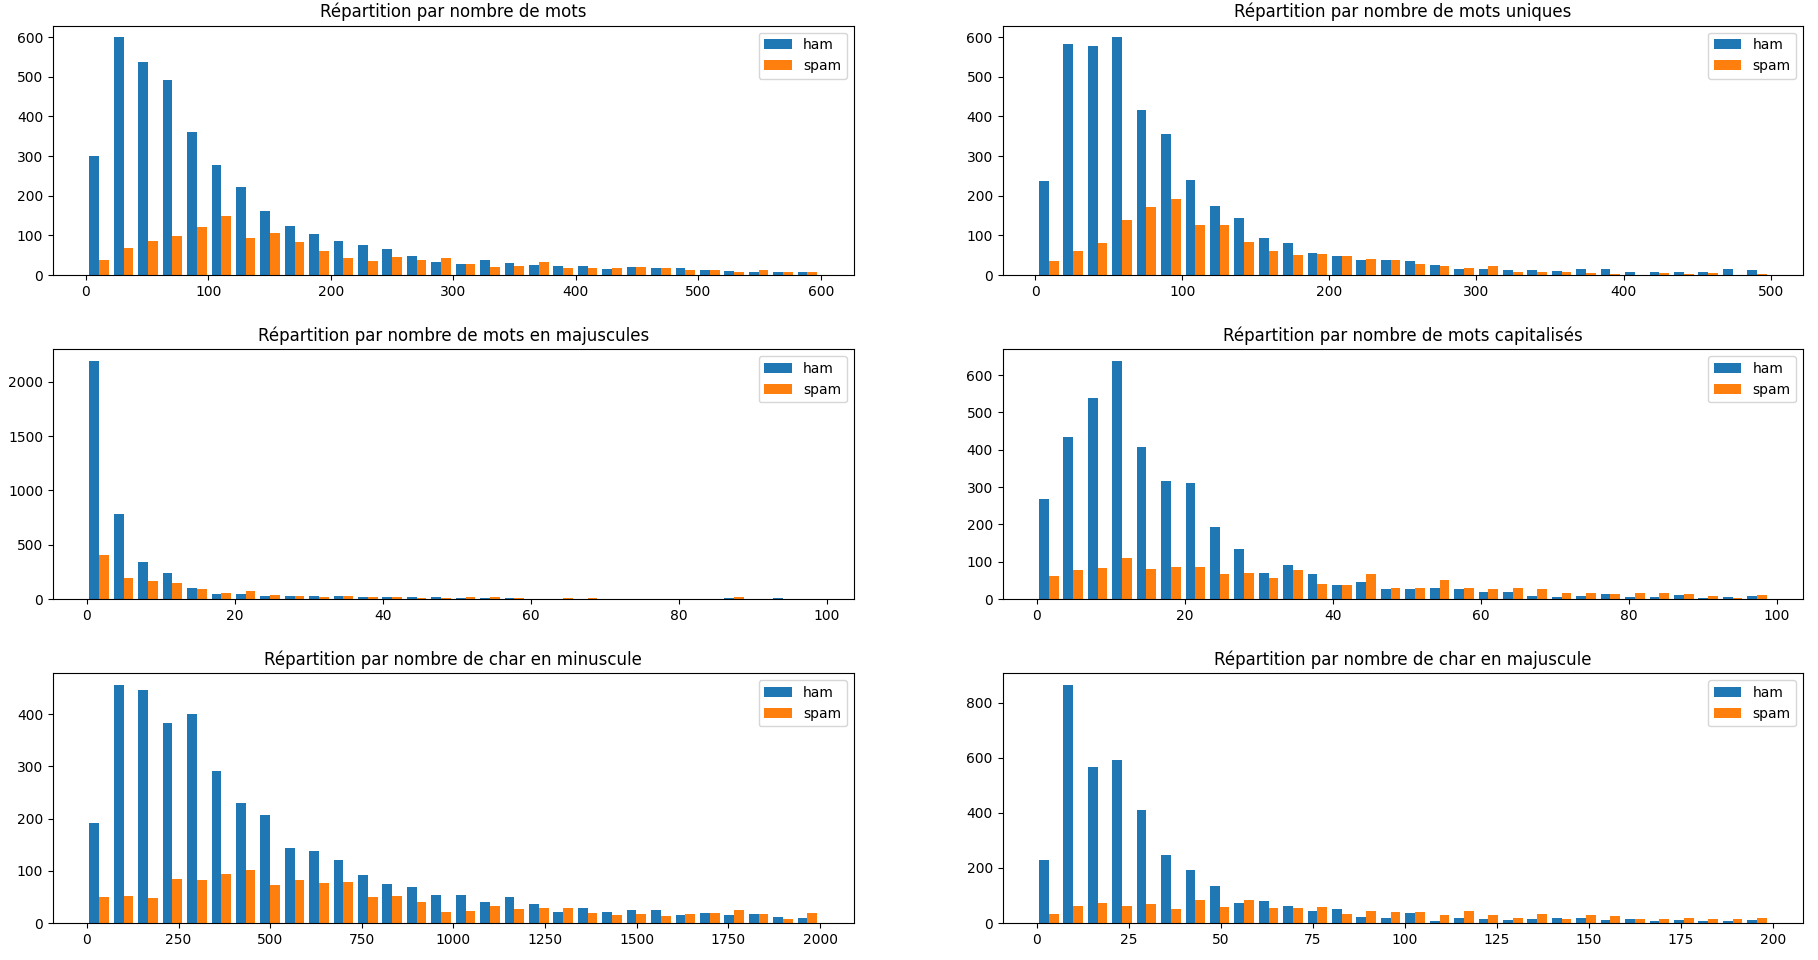
\includegraphics[width=\linewidth]{img/p2mots.png}
					\caption{Distribution des données de mots selon la catégorie du mail}
					\label{fig:p2mots}
				\end{figure}
				Concernant les distributions des mails visibles dans la Figure \ref{fig:p2mots} on remarque que les Ham se concentrent généralement vers des métriques basses puis l'effectif se réduit à mesure que la valeur de la métrique augmente. Les Spam quand à eux ont plus tendance à suivre une distribution de type normale ou uniforme.
				
		
		
		\paragraph{Statistiques des ponctuations}
			\begin{table}[htbp]
				\centering
				\captionof{table}{Statistiques sur les ponctuations} \label{tab:sponct}
				\resizebox{\columnwidth}{!}{\begin{tabular}{|l|c|c|c|c|c|c|c|c|c|c|c|c|}
					\hline
								& \multicolumn{3}{|c|}{points} & \multicolumn{3}{|c|}{virgules} & \multicolumn{3}{|c|}{exclamations} & \multicolumn{3}{|c|}{interrogations} \\
								& Global		& Ham 	& Spam 	& Global		& Ham	& Spam	& Global		& Ham	& Spam	& Global		& Ham	& Spam	\\
					\hline
					moyenne		& 14			& 12		& 20		& 12			& 11		& 16		& 2			& 0.7	& 5.9	& 1			& 0.9	& 1.3	\\
					\hline
					écart-type	& 35			& 30		& 46		& 37			& 31		& 50		& 7			& 5		& 10		& 2			& 2		& 3		\\
					\hline
					minimum		& 0			& 0		& 0		& 0			& 0		& 0		& 0			& 0		& 0		& 0			& 0		& 0		\\
					\hline
					25\%			& 3			& 3		& 3		& 2			& 2		& 2		& 0			& 0		& 1		& 0			& 0		& 0		\\
					\hline
					médiane		& 6			& 5		& 9		& 5			& 4		& 6		& 0			& 0		& 3		& 0			& 0		& 0		\\
					\hline
					75\%			& 13			& 11		& 18		& 10			& 9		& 14		& 2			& 1		& 7		& 1			& 1		& 1		\\
					\hline
					maximum		& 848		& 848	& 643	& 1268		& 890	& 1268	& 343		& 343	& 92		& 79			& 79		& 58		\\
					\hline
				\end{tabular}}
			\end{table}
			
			Le tableau \ref{tab:sponct} des données de ponctuation donne l'information que les textes des Spam utilisent plus de signes de ponctuation que les Ham. Il faut relever que l'utilisation des points d'interrogation est anecdotique pour les deux catégories.  	
			
			\begin{figure}[H]
				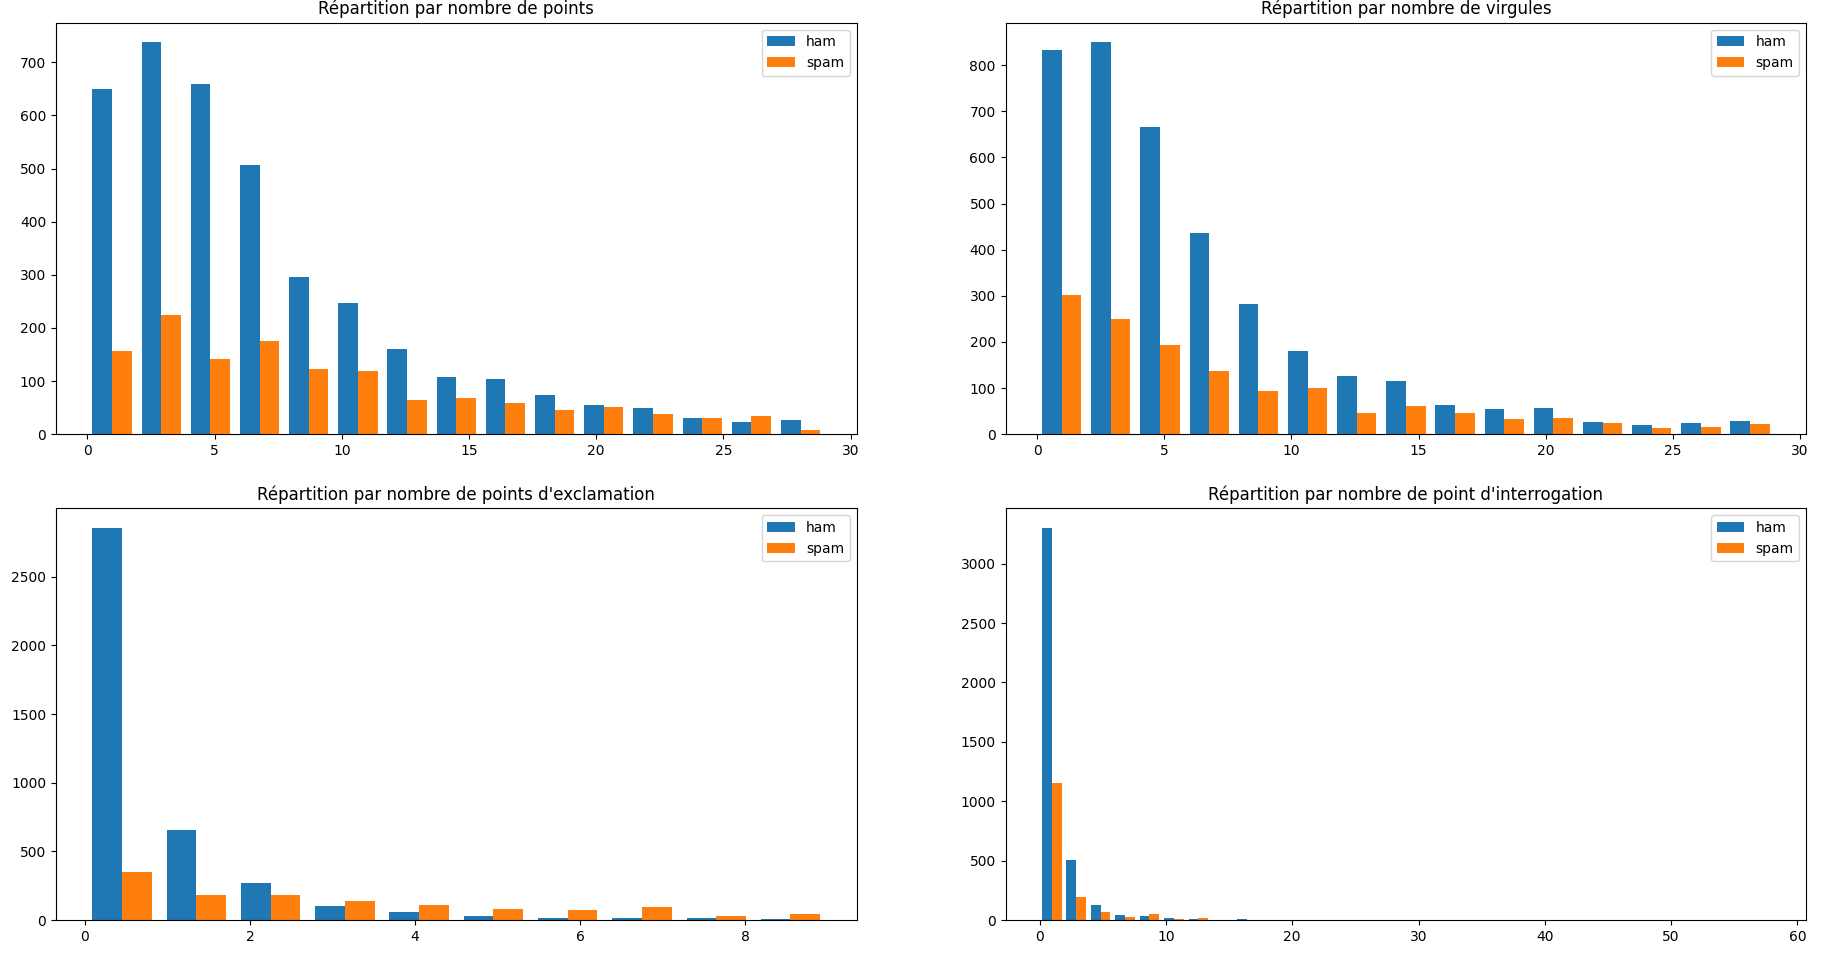
\includegraphics[width=\linewidth]{img/p2ponct.png}
				\caption{Distribution des données de la ponctuation selon la catégorie du mail}
				\label{fig:p2ponct}
			\end{figure}	
			Les schéma de la Figure \ref{fig:p2ponct} montrent un comportement similaire pour les deux catégories avec le nombre de points, de virgule et de point d'interrogation. 
			Seule la répartition des effectifs de spam pour le nombre de point d'exclamation semble ne pas suivre le même cheminement et semble rester uniforme. 
			
			
			
		\paragraph{Statistiques des espaces et des lignes}
			\begin{table}[htbp]
				\centering
				\captionof{table}{Statistiques sur les espaces et les lignes} \label{tab:sspace}
				\resizebox{\columnwidth}{!}{\begin{tabular}{|l|c|c|c|c|c|c|c|c|c|c|c|c|}
					\hline
								& \multicolumn{3}{|c|}{tabulations} & \multicolumn{3}{|c|}{espaces} & \multicolumn{3}{|c|}{lignes} & \multicolumn{3}{|c|}{lignes vides} \\
								& Globale	& Ham 	& Spam 	& Globale	& Ham	& Spam	& Globale	& Ham 	& Spam 	& Globale	& Ham	& Spam	\\
					\hline
					moyenne		& 2			& 2		& 3		& 287		& 240	& 411	& 65			& 57	 	& 86	 	& 15			& 13		& 19		\\
					\hline
					écart-type	& 29			& 32		& 19		& 874		& 917	& 733	& 137		& 144 	& 113 	& 44			& 50		& 22		\\
					\hline
					minimum		& 0			& 0		& 0		& 1			& 2		& 1		& 1			& 1	 	& 1	 	& 0			& 0		& 0		\\
					\hline
					25\%			& 0			& 0		& 0		& 55			& 45		& 99		& 21			& 19	 	& 28	 	& 6			& 6		& 8		\\
					\hline
					médiane		& 0			& 0		& 0		& 114		& 95		& 196	& 34			& 30	 	& 52	 	& 9			& 8		& 13		\\
					\hline
					75\%			& 0			& 0		& 0		& 255		& 196	& 435	& 61			& 48	 	& 97	 	& 14			& 12		& 23		\\
					\hline
					maximum		& 1118		& 1118	& 379	& 36350		& 36350	& 11436	& 6320		& 6320 	& 1695 	& 2882		& 2882	& 291	\\
					\hline
					
				\end{tabular}}
			\end{table}
			
			Le tableau \ref{tab:sspace} regroupe les données des espace vide et le calcul du nombre de lignes. On remarque que les tabulations ne sont pas utilisées, sauf en grande quantité. Il pourrait être intéressant de voir si cet élément peut être utiliser pour détecter les documents générant des valeurs aberrantes. Pour ce qui est du nombre d'espaces, de lignes et de lignes vide, la moyenne des Spam est approximativement le double de celle des Ham.
			
			\begin{figure}[H]
				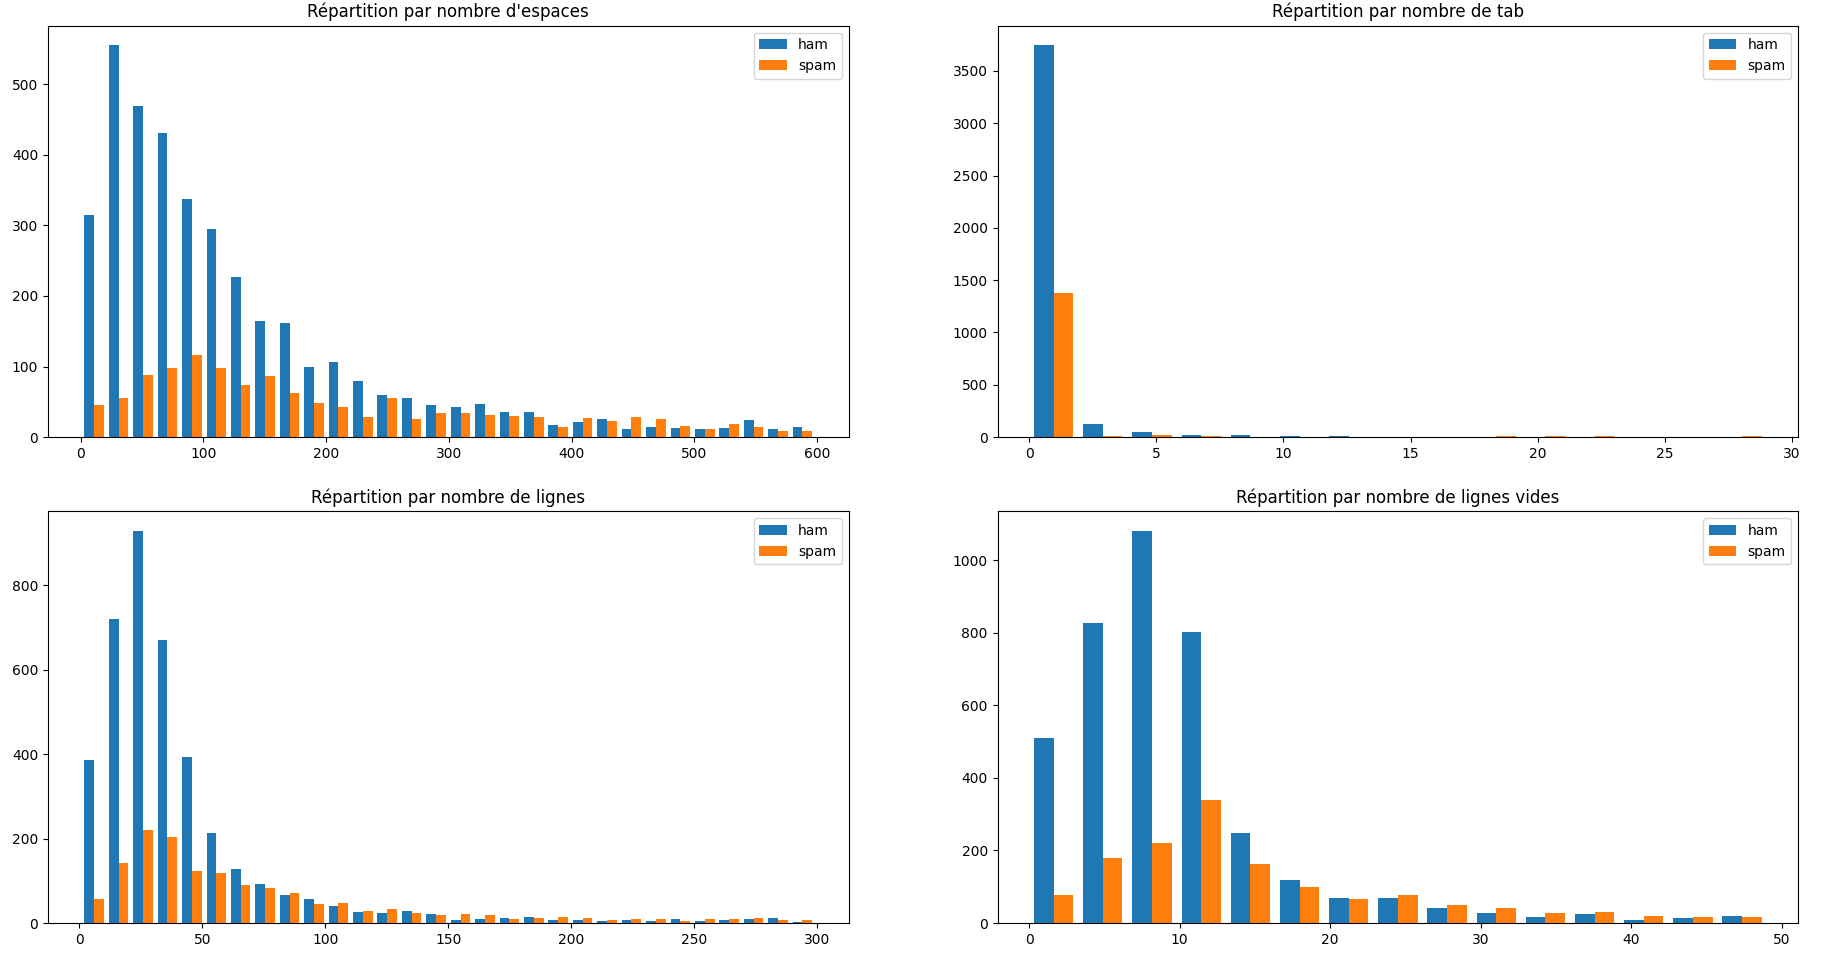
\includegraphics[width=\linewidth]{img/p2lignes.png}
				\caption{Distribution des données de lignes et espaces selon la catégorie du mail}
				\label{fig:p2lignes}
			\end{figure}	
		
		On peut voir dans les histogrammes de la Figure \ref{fig:p2lignes} que les mails se répartissent de manière relativement normale pour le comptage du nombre de lignes et de lignes vides pour des valeurs faibles. Puis à mesure que la valeur augmente, l'effectif semble se réduire de manière linéaire. La répartition du nombre d'espace ressemble fortement à la répartition du nombre de mots. Il est possible que le nombre d'espaces soit corrélé au nombre de mots.  
		
		\paragraph{Distribution de Zipf} Cette distribution est une loi empirique qui permet de décrire un classement des mots selon leur fréquence d'apparition. Les fonctions utilisées pour la mise en œuvre de cette distribution ont été réalisées par mes soins. L'annexe \ref{sec:devZipf} détaille le développement de cette fonctionnalité.  
		
			Les données suivantes montre la représentation de cette distribution pour l'ensemble du corpus.
			\begin{figure}[H]
  				\centering
  				\begin{subfigure}[b]{0.3\linewidth}
    					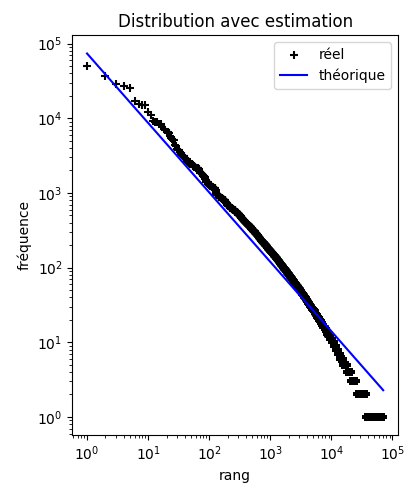
\includegraphics[width=\linewidth]{img/zipfGlobal.png}
    					\caption{Ham + Spam}
  				\end{subfigure}
  				\begin{subfigure}[b]{0.3\linewidth}
    					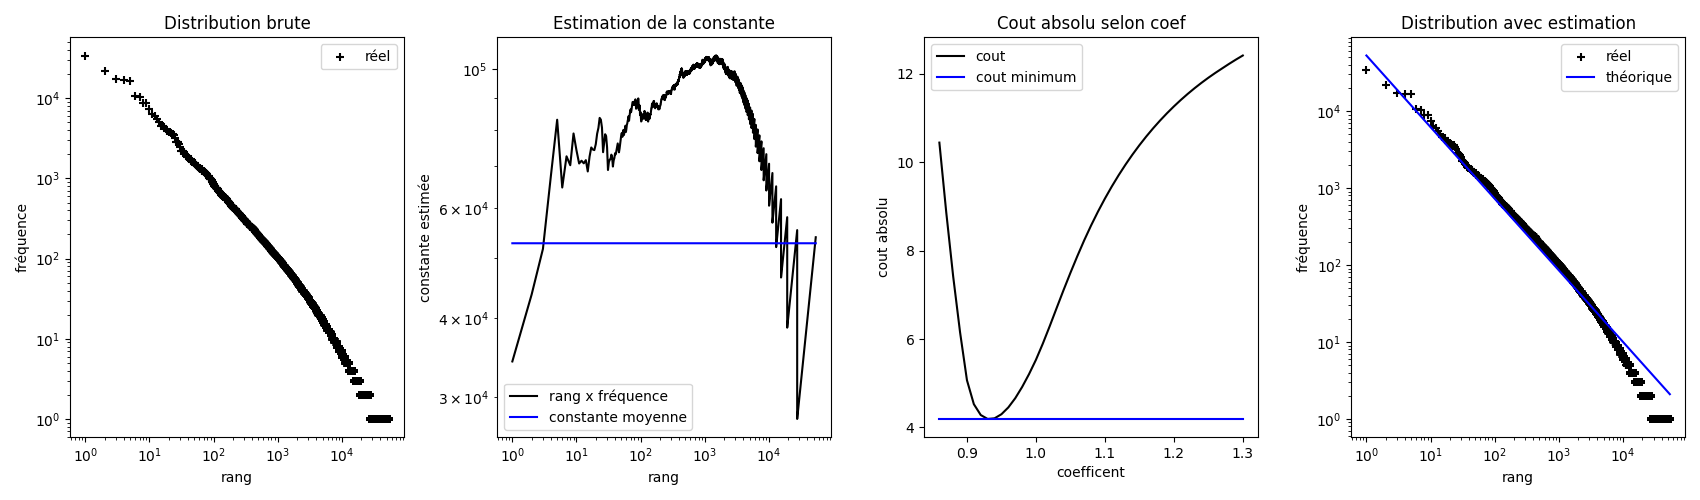
\includegraphics[width=\linewidth]{img/zipfHam.png}
    					\caption{Ham}
  				\end{subfigure}
  				\begin{subfigure}[b]{0.3\linewidth}
  					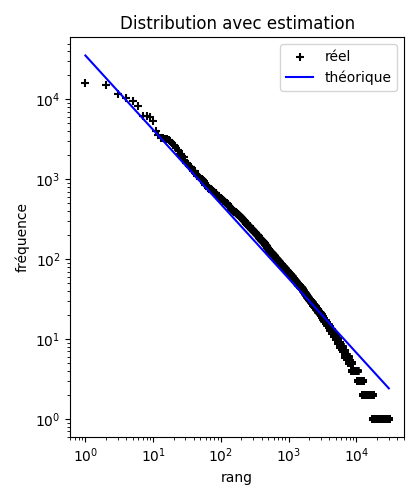
\includegraphics[width=\linewidth]{img/zipfSpam.png}
  					\caption{Spam}
				\end{subfigure}  				
  				\label{fig:coffee}
			\end{figure}	
			
			On voit dans les graphiques ci dessus que les corpus Ham, Spam et l'association des deux respectent une distribution zipfienne.
			
			\begin{table}[H]
			\centering
				\begin{tabular}{|l|c|c|c||c|c|c|}
					\hline
								& constante & coefficient & erreur moyenne & hapax & hapax/vocab & hapax/total \\
					\hline
					Ham + Spam  & 73746.97  & 0.93        & 6.37	             & 33666 & 0.47              & 0.02 \\
					\hline
					Ham 		    & 52712.40  & 0.93        & 4.19              & 26231 & 0.48              & 0.03 \\
					\hline
					Spam		    & 35485.13  & 0.93        & 4.84              & 12396 & 0.40              & 0.02 \\
					\hline
				\end{tabular}
			\end{table}
			
			On remarque à partir du tableau ci dessus que la constante estimée est plus importante dans les corpus Ham que dans le corpus Spam. La constante des Ham (52712) est assez proche de la constante moyenne découverte avec le corpus de Brown lors du développement de cette méthode (56525). Il est possible d'émettre l'hypothèse que le vocabulaire des Ham est plus fournis. On remarque également que le taux d'hapax dans le vocabulaire des Ham est de 48\% alors que cette proportion est de 40\% pour les Spam.    
			
			
			\paragraph{Distribution de Zipf par message} Le processus appliqué pour le calcul de la distribution de Zipf sur les différent corpus a été utilisé sur chaque mail individuellement. Il a alors été possible d'ajouter ces données (constante, coefficient, taux d'erreur, nombre d'hapax et ratio d'hapax) pour chaque mail. Le résultat de ce traitement est détaillé dans le Tableau \ref{tab:zipf} et dans la Figure \ref{fig:p2zpif}.
			
							\begin{table}[H]
					\centering
					\captionof{table}{Statistiques sur les données des calculées de Zipf et Hapax} \label{tab:zipf}
					\resizebox{\columnwidth}{!}{\begin{tabular}{|l|c|c|c|c|c|c|c|c|c|c|c|c|}
						\hline
									& \multicolumn{2}{|c|}{constante} & \multicolumn{2}{|c|}{coefficient} & \multicolumn{2}{|c|}{taux d'erreur} & \multicolumn{2}{|c|}{hapax} & \multicolumn{2}{|c|}{ratio vocabulaire} & \multicolumn{2}{|c|}{ratio texte}\\
									& Ham 	& Spam 	& Ham	& Spam	& Ham 	& Spam 	& Ham	& Spam & Ham 	& Spam 	& Ham	& Spam	\\
						\hline
						moyenne		& 66		& 102	& 1.21	& 1.19	& 1.37	& 1.54	& 87.7	& 111.53	& 0.83	& 0.72	& 0.67	& 0.52	\\
						\hline
						écart-type	& 115	& 141	& 0.08	& 0.07	& 0.24	& 0.41	& 123.8	& 123.4	& 0.12	& 0.21	& 0.20	& 0.22	\\
						\hline
						minimum		& 2		& 1		& 0.86	& 0.86	& 0.44	& 0		& 0		& 0		& 0		& 0		& 0		& 0	 	\\
						\hline
						25\%			& 21		& 39		& 1.16	& 1.14	& 1.26	& 1.37	& 35		& 51		& 0.77	& 0.71	& 0.52	& 0.40 	\\
						\hline
						médiane		& 36		& 63		& 1.22	& 1.19	& 1.37	& 1.46	& 57		& 80		& 0.84	& 0.77	& 0.67	& 0.54 	\\
						\hline
						75\%			& 65		& 112	& 1.29	& 1.26	& 1.46	& 1.57	& 93		& 136	& 0.91	& 0.83	& 0.83	& 0.67 	\\
						\hline
						maximum		& 2311	& 1866	& 1.30	& 1.30	& 3.49	& 3.49	& 3552	& 1690	& 1		& 1		& 1		& 1	 	\\
						\hline
						
					\end{tabular}}
				\end{table}
				Le tableau \ref{tab:zipf} montre que les constantes estimées sont globalement plus importantes dans les spams. Le coefficient est plus élevé dans les Ham. Cependant il est à noté que la moyenne des coefficient pour les Ham ($1.21$) et pour les Spam ($1.19$) est assez supérieure au coefficient estimé pour tout le corpus ($0.93$). On remarque également pour le coefficient que la valeur se rapproche rapidement de $1.30$ qui est la limite haute fixée pour l'estimation du coefficient. 
				
				Le taux d'erreur, qui correspond à la moyenne de l'écart absolu entre la valeur réelle et estimée de la constante, est plus élevé dans les spam ($1.54$). Mais cette valeur reste inférieure à celle observée  pour l'ensemble du corpus. Cela peut s'expliquer par un écart de fréquence moins important entre le mots les plus présents et les moins présents.
				
				Le calcul des hapax semble plus parlant mail par mail que dans la globalité du corpus. On remarque effectivement un écart de 15 points entre la moyenne des hapax dans les textes des Ham ($67\%$) que dans ceux des Spam ($62\%$). En comparaison cet écart n'est que de 1 point sur l'ensemble de chaque corpus.
				
				\begin{figure}[H]
					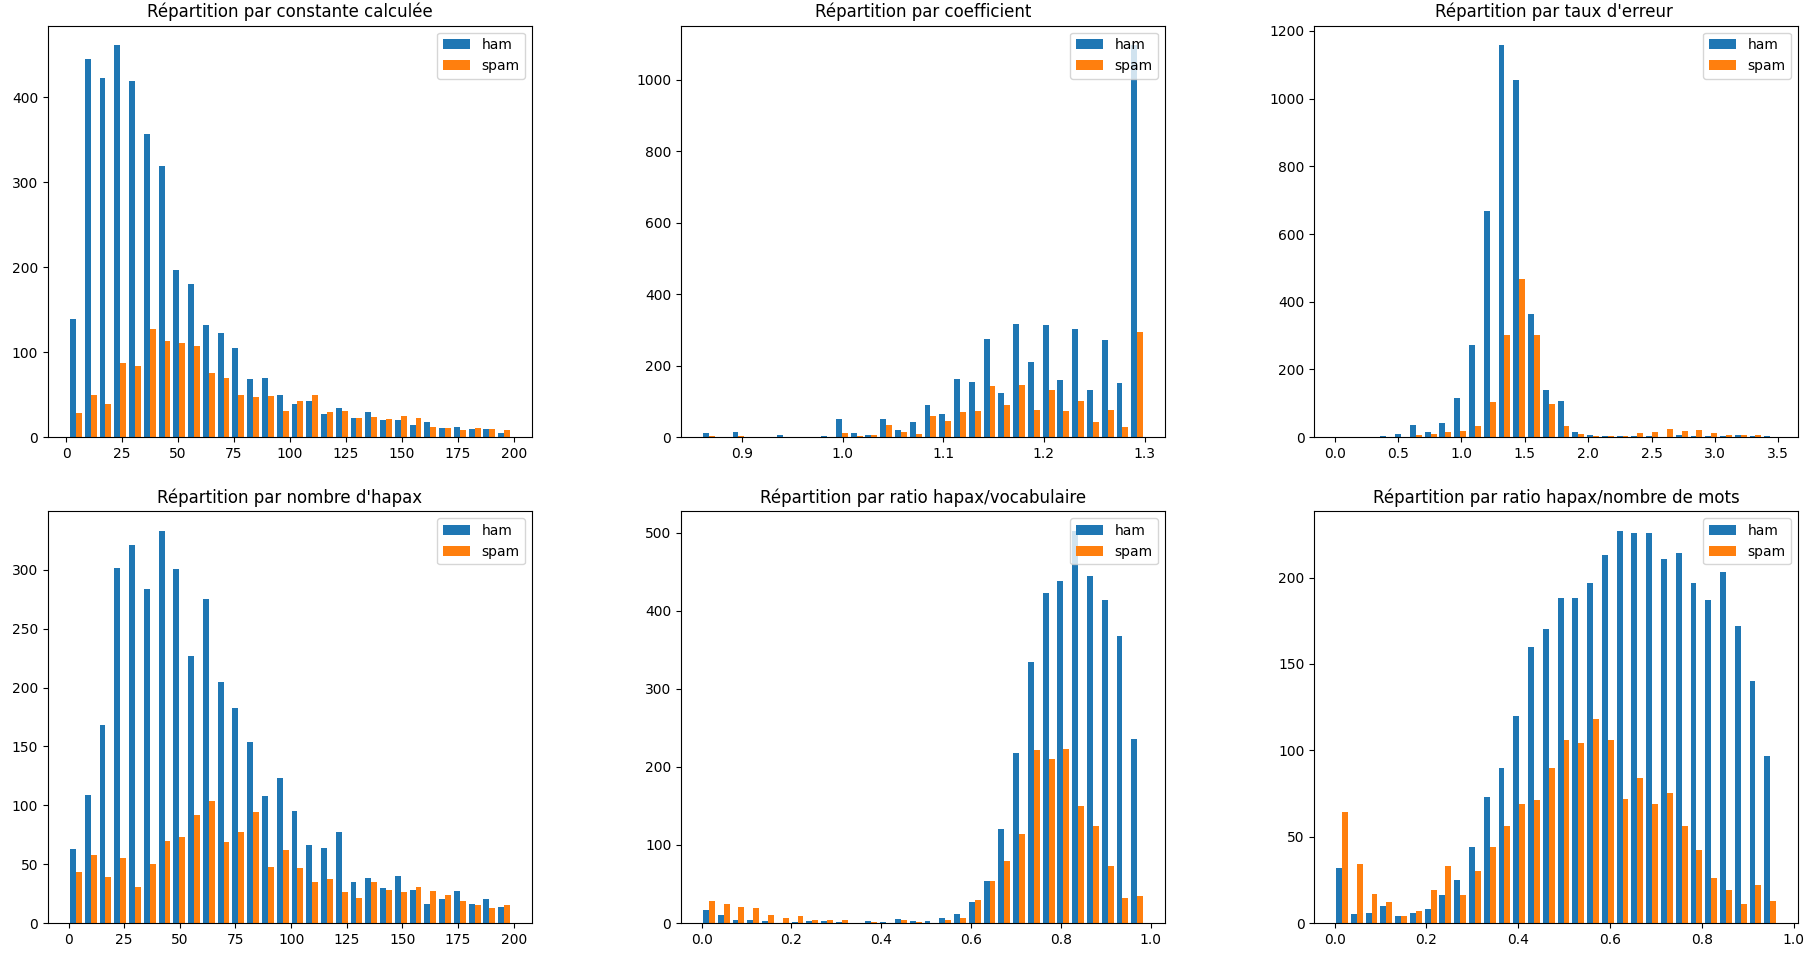
\includegraphics[width=\linewidth]{img/p2zipf.png}
					\caption{Distribution des données de Zipf selon la catégorie du mail}
					\label{fig:p2zpif}
				\end{figure}	
				
				On voit dans les schéma de la Figure \ref{fig:p2zpif} que les Ham se concentre également dans les valeurs basses de la constante. Les Spams semblent plus dispersés pour cette métrique.
				
				Le nombre d'hapax lui semble suivre une distribution normale pour les Ham. Pour cette métrique la répartition est plus diffuse. 

				Les ratio du nombre d'hapax par rapport au vocabulaire et à l'ensemble du corps du mail ont une distribution normale sauf pour des valeurs marginales entre $0\%$ et $20\%$. Il est intéressant de remarquer que les spam sont majoritaires dans cette tranche alors que le nombre de Spam est nettement inférieur au nombre de Ham dans le data set	(70/30).		
				
				Le pic du taux d'erreur des Ham (1.4) est effectivement inférieur à celui des Spam (1.5). On remarque également un regroupement de Spam avec un taux d'erreur compris entre (2.3 et 3).
				
				Enfin il semblerait que le coefficient de chaque type gravite autour de la médiane, avec base assez large. Le pic en bout de graphique peut être ignoré car il correspond à la limite haute de la recherche de coefficient bornée entre 0.8 et 1.30. augmenter cette limite impliquerait d'augmenter les temps que calcul qui ne semble pas justifié dans ce cas. Moins de $25\%$ des documents ont été classés avec un coefficient supérieur à $1.29$.
				
				
			\paragraph{Matrice de corrélation}
				La corrélation entre 2 variables permet de voir l'interdépendance entre elles. Il est alors possible de voir si leurs augmentations ou diminutions sont de nature à être liées. Cette relation peut dans certain cas montrer une relation de cause à effet. 
				
				Le calcul des coefficients présentés dans la matrice de la Figure \ref{fig:corr} utilise la méthode de corrélation linéaire de Pearson.
				Il s'agit ici de calculer le ratio ($r$) de la covariance entre 2 variables par le produit de leurs écart-types.
				
				\begin{eqnarray*}
					r_{X,Y} &=& \frac{cov(X,Y)}{\sigma_{X}\sigma_{Y}}\\
					r_{X,Y} &=& \frac{\sum_{i=1}^{n}(x_{i}-\overline{x})(y_{i}-\overline{y})}{\sqrt{\sum_{i=1}^{n}(x_{i}-\overline{x})^{2}}\sqrt{\sum_{i=1}^{n}(y_{i}-\overline{y})^{2}}}
				\end{eqnarray*}
				
				Une corrélation forte sera proche des bornes $1$ et $-1$. Une corrélation faible sera proche de $0$. 
			
				\begin{figure}[H]
					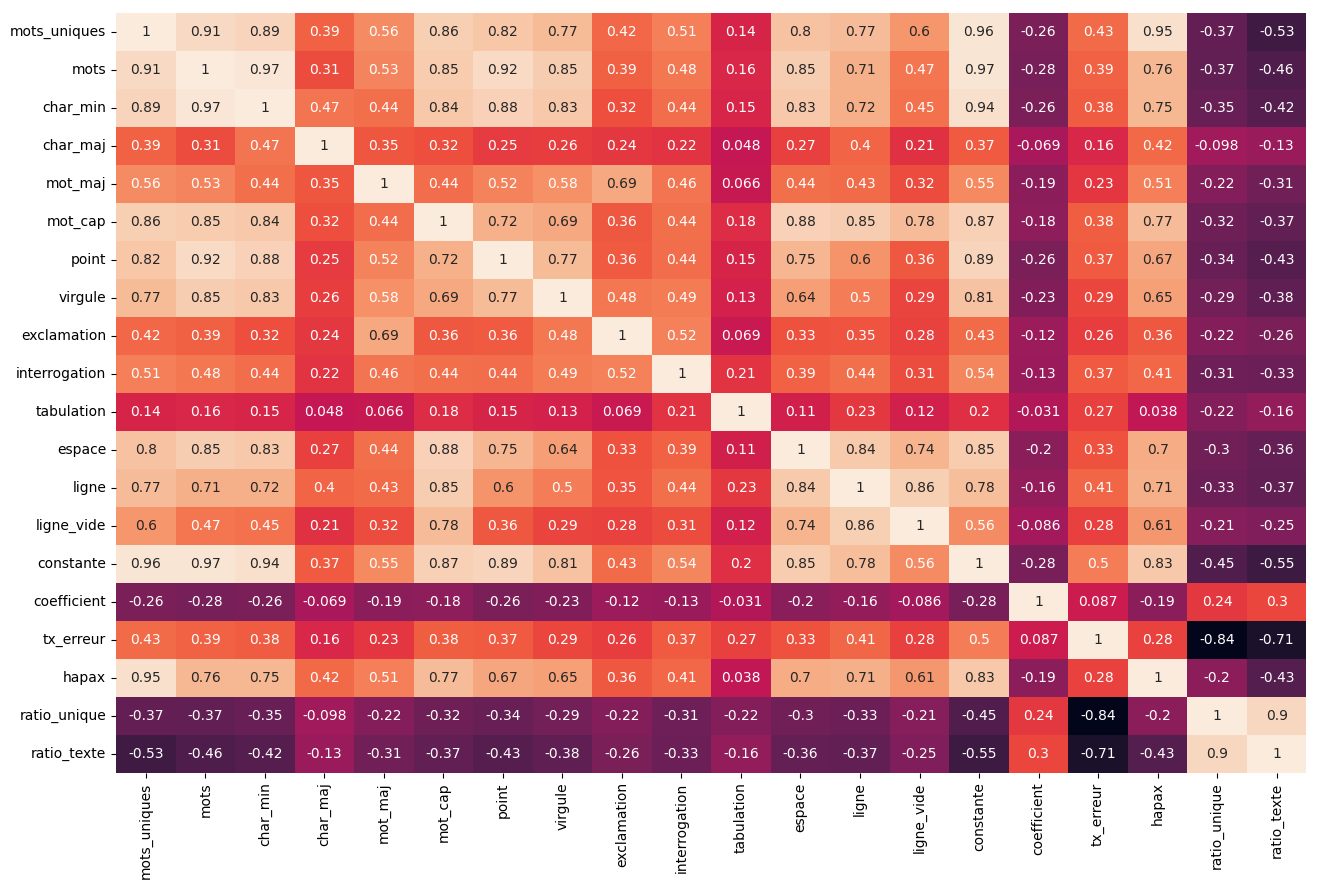
\includegraphics[width=\linewidth]{img/p2corr.png}
					\caption{Matrice de corrélation des métriques}
					\label{fig:corr}
				\end{figure}	
				
				On peut remarquer que les nombre de mots, de caractères en minuscule, de points et de virgules sont fortement corrélés.
				On voit également que certaines métriques sont quasiment indépendante de la plus part des autres variables:
				\begin{itemize}
					\item nombre de caractères en majuscules
					\item nombre de mots en majuscules
					\item nombre de point d'exclamation
					\item nombre de point d'interrogation
					\item nombre de tabulation
					\item coefficient Zipf déterminé
					\item ratio d'hapax dans le vocabulaire
					\item ratio d'hapax dans tout le texte
				\end{itemize}
				
				Les variables dénombrant les espaces et les lignes (vides ou non) sont faiblement liées aux signes de ponctuations.
			
			
			\paragraph{Résumé} L'analyse de l'utilisation des données des mots permet me mettre en lumière les points suivants :
			\begin{itemize}
				\item Les Spam sont généralement plus long que les Ham
				\item On retrouve plus de caractères en majuscules dans les Spam que dans les Ham
				\item Les nombres de mots et de mots uniques sont fortement corrélés
			\end{itemize}
			
			Les données sur l'utilisation des ponctuations ne montre pas d'écart majeur entre les Ham et les Spam sur l'utilisation des points et des virgule. Cependant l'utilisation des points d'exclamation est nettement plus forte dans les Spam. \\
			L'utilisation de point d'exclamation et de majuscule est susceptible d'induire une notion d'urgence chez le lecteur.\\
			
			Les données des lignes et des espaces ne permettent de faire une différence franche entre les Ham et les Spams au regards des autres données.\\ 
			
			Globalement, les Ham et les Spam respectent les principes de la distribution de Zipf. Le coefficient est identique pour chacun des deux corpus. La constante et le nombre d'Hapax plus importantes pour les Ham s'expliquent par un nombre de document largement supérieur.
			 
			En regardant les données de la distribution de Zipf appliquée à chaque mail on remarque un coefficient moyen plus élevé et qui semble plus précis pour les Ham. Il est également notable que les mots se répètent moins dans les messages Ham.\\
			
			
			En conclusion, on peut supposer les faits suivants : 
			\begin{itemize}
				\item Le vocabulaire d'un Ham est plus fourni que celui d'un Spam.
				\item Il y a plus de mots dans un Spam.
				\item Un Spam aura probablement une construction induisant une notion d'urgence.
			\end{itemize}
			
		
	\subsection{Traitement du langage}
		 Dans cette section nous aborderons des traitements du langage naturel qui vont être employés afin de tenter de détecter des similitudes dans les thèmes abordés dans les mails de chaque catégorie. Pour cela nous allons transformer les messages en un ensemble de clé/valeur avec le mot ainsi que sa fréquence dans le document. Les données récoltées seront utilisées pour vectoriser les document avec la méthode TF-IDF.
		 
			
		 \paragraph{Schéma d’exécution}
		 	Les corps de mail brut vont être récupérés dans la base de données ElasticSearch.\\ 
		 	La première étape vise à vérifier que le message est déjà passé par l'étape de traitement de la phase 1 et qu'il est présent dans la base de données PSQL. Pour le moment, l'absence du message dans la base PSQL termine le traitement NLP du message. Une évolution possible serait de déclencher automatiquement les traitements précédents. \\
		 	La deuxième étape permet d'éviter que le traitement d'un même message s'effectue plusieurs fois. cela est possible en vérifiant la présence de l'identifiant de message dans la table \emph{nlp\_status}.
		 	Dans L'étape de lemmatisation nous allons utiliser le moteur de \emph{StandfordNLP}\cite{manning-EtAl:2014:P14-5}lcite{qi2020stanza}. Les processus utilisés sont décrits plus bas.\\
		 	Le calcul de la fréquence des mots utilise le code développé lors la recherche de la distribution de Zipf. A l'issue de cette phase les données de fréquence pour chaque mots et messages sont mis en base.
		 
		 \begin{figure}[H]
				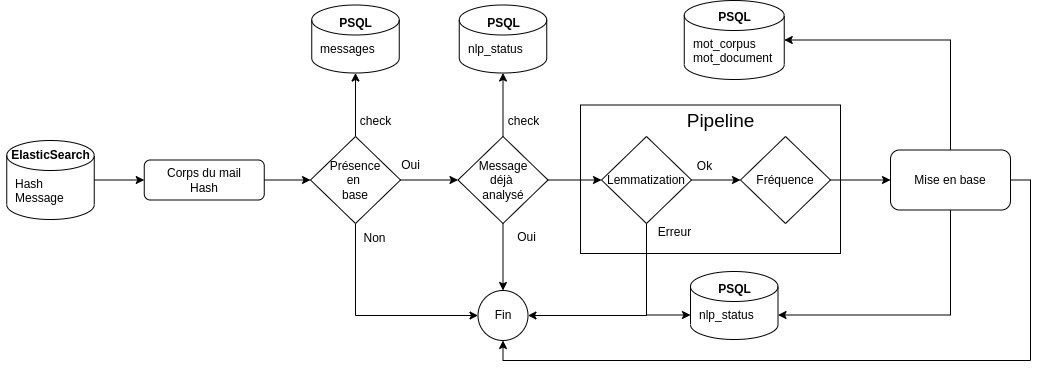
\includegraphics[width=\linewidth]{img/p2schema.png}
				\caption{Schéma du déroulement des instructions}
		\end{figure}
		 
		 
		 \paragraph{Modification de la base de données}
		 	Afin de stocker les informations générées pendant cette phase 3 nouvelles tables vont être ajoutée à la base de données PSQL existante:
		 	\begin{enumerate}
		 		\item \textbf{mot\_corpus} - Cette table regroupe les mots du corpus
		 			\begin{itemize}
		 				\item id\_mot - clé primaire du mot dans la base
		 				\item mot - valeur du mot
		 				\item freq\_corpus - fréquence du mot dans le corpus
		 				\item freq\_doc\_all - nombre total de document avec le mot
		 				\item freq\_doc\_spam - nombre de spam avec le mot
		 				\item freq\_doc\_ham - nombre de ham avec le mot
		 			\end{itemize}
		 		\item \textbf{mots\_document} - Table faisant la liaison entre les mot et les messages
		 			\begin{itemize}
		 				\item id\_message - identifiant unique du message dans la base
		 				\item id\_mot - identifiant unique du mot dans la base
		 				\item occurence - nombre d'occurence de mot dans le message
		 			\end{itemize}
		 		\item \textbf{nlp\_status} - enregistrement de résultat du statut du traitement NLP
		 			\begin{itemize}
		 				\item id\_message - identifiant unique du message dans la base
		 				\item success - réussite ou échec
		 				\item raison - raison de l'échec
		 			\end{itemize}
		 	\end{enumerate}
		 	
		 	La table \textbf{nlp\_status} va permettre de ne pas traiter plusieurs fois le même message. Le module de traitement NLP standford est susceptible de généré des erreurs lors du traitement de certains messages. Ces messages seront exclus du traitement. \\
		 	
		 	Les erreurs rencontrées pour la fonction lemmatise sont:
		 	\begin{itemize}
		 		\item TypeError - POURQUOI ?????????????
		 		\item OutOfMemoryError - POURQUOI ?????????????
		 	\end{itemize}
		 	
			\begin{figure}[H]
				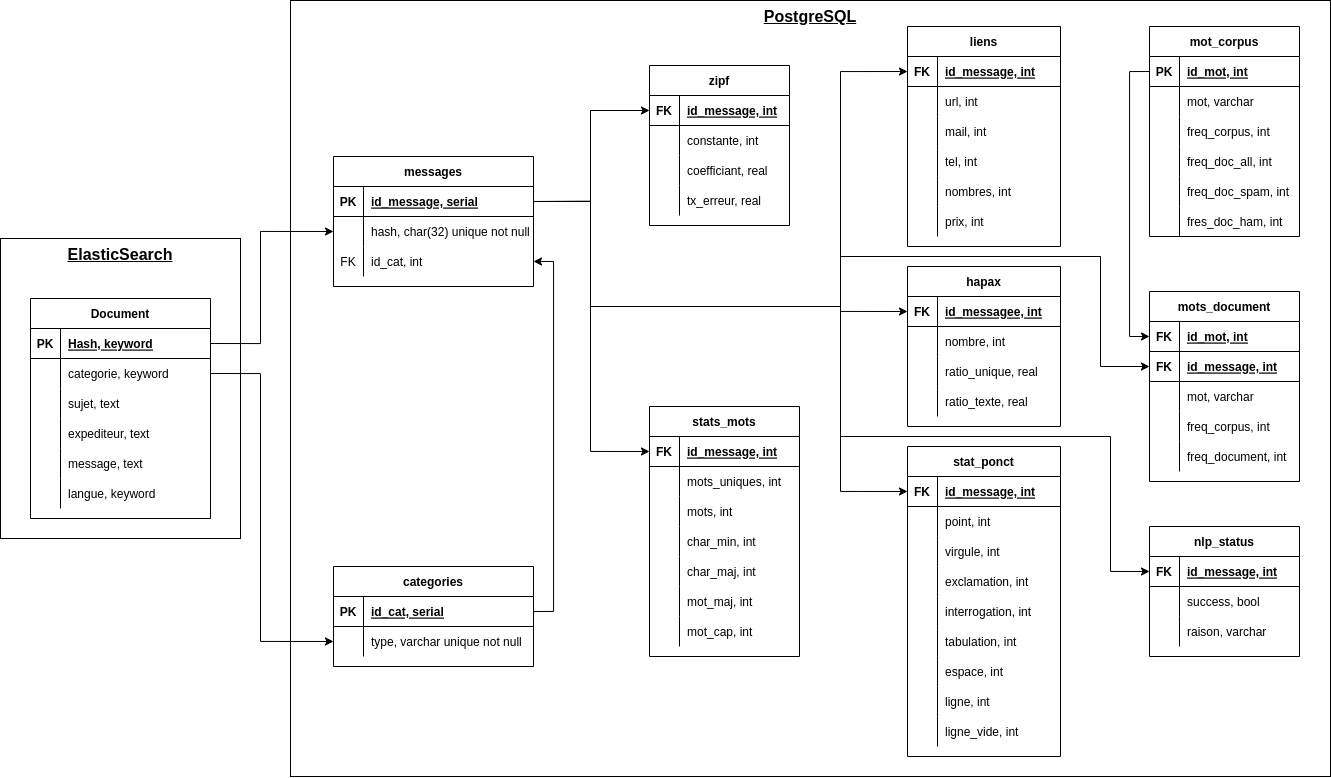
\includegraphics[width=\linewidth]{img/p2Bdd.png}
				\caption{Schéma des bases de données pour accueillir les données NLP}
			\end{figure}
			
			
			Les nouvelles tables ont été ajoutées en utilisant les fonctions présentées dans l'annexe \ref{PSQL} avec le mapping suivant:
			\begin{lstlisting}[title=Mapping nouvelles tables]
{
  "mail_features_prod": {
    "mot_corpus": {
      "id_mot": ["SERIAL", "PRIMARY KEY"],
      "mot": ["VARCHAR", "UNIQUE", "NOT NULL"],
      "freq_corpus": ["INT"],
      "freq_doc_all": ["INT"],
      "freq_doc_spam": ["INT"],
      "freq_doc_ham": ["INT"]
    },
    "mots_document": {
      "id_message": ["INT"],
      "id_mot": ["INT"],
      "occurrence": ["INT"],
      "pk": ["id_message", "id_mot"],
      "fk": {
        "fk_message": ["id_message", "messages(id_message)", "SET NULL"],
        "fk_mot": ["id_mot", "mot_corpus(id_mot)", "SET NULL"]
      }
    },
    "nlp_status": {
      "id_message": ["INT"],
      "success": ["BOOL"],
      "raison": ["VARCHAR"],
      "pk": ["id_message"],
      "fk": {
        "fk_message": ["id_message", "messages(id_message)", "SET NULL"]
      }
    }
  }
}
			\end{lstlisting}
			
			
		\subsubsection{Lemmatisation}
			La lemmatisation d'un texte vise à réduire la taille d'un texte en ramenant chaque mot à la forme du mot présente dans le dictionnaire. Ce traitement permet donc de compter le nombre d'occurence d'un mot sans se soucier de sa forme ou des modifications grammaticales appliquées lors de la rédaction du texte. A l'issue de ce traitement nous serons en mesure de connaître les mots les plus utilisés dans les corps des mails et tenter de déterminer les thèmes les plus récurrents.  
			Dans ce projet, nous allons utiliser le moteur de lemmatisation de \emph{StandfordNLP}\cite{manning-EtAl:2014:P14-5}\cite{qi2020stanza}
			Les traitements nécessaire pour arriver à une lemmatisation sont :
			\begin{enumerate}
				\item Tokenisation : Séparer les phrases en token. Ici chaque token correspond à un mot ou à une ponctuation.
				\item Multi-Word Token Expansion : Ce traitement n'est pas nécessaire en anglais selon la documentation \emph{Stanza}. Ce traitement permet d'étendre un token s'il correspond à une contraction de plusieurs terme. Par exemple en français le terme \emph{du} sera transformé en \emph{de le}.
				\item Part of Speech Tagging: Cette opération vise à marquer chaque mot du texte avec sa position grammaticale dans la phrase qui le contient et va permettre d'effectuer le transfert vers le lexème correspondant.
			\end{enumerate}
			
			L'initialisation de la pipeline de lemmatisation de Stanza se fait en appelant la classe \emph{Pipeline} avec les arguments de langage et de processus dans l'ordre d'utilisation. 
			A cette étape j'ajoute 2 filtres. Le premier va me permettre de ne conserver que les mots avec des lettres.
			La deuxième étape permet de retirer les stopwords en anglais qui ne permettent pas d'analyser le sens du message.\\
			La dernière étape avant la mise en base permet de compter la fréquence de chaque mot dans le texte
			\begin{lstlisting}[title=Pipeline de lemmatisation, language=python]
import nltk
import stanza
import stats

nltk.download("stopwords")
en_stopwd = set(stopwords.words('english'))
pipe = stanza.Pipeline(lang='en', processors='tokenize,mwt,pos,lemma')
pat = re.compile(r'\w+')

def lemmatise(message, stopwds, pipeline, pattern):
    doc = pipeline(message)
    lemma = [mot.lemma for phrase in doc.sentences for mot in phrase.words]
    return [lem.lower() for lem in lemma if re.match(pattern, lem) and lem.lower() not in stopwds]
  
stats.frequence_mot(lemmatise(value, en_stopwd, pipe, pat))
			\end{lstlisting}

			Ci dessous un exemple des étapes du traitement sur un message de la base
			\begin{verbatim}
>>> print(value)
Heres the hottest thing in DVDs. Now you can make a personal backup
copy of a DVD right onto CDR.  Our Hot new software easily takes you through
the steps to make a copy of your own DVDs.
NOW INCLUDED FOR FREE! Copy PLAYSTATION, MUSICMPs and all Software.
 Step by Step Interactive Instructions 
 All Software Tools Included On CD 
 No DVD Burner Required 
 FREE Live Technical Support 
  Day Risk Free Trial Available 
 FREE Dvd Movie of your choice LIMITED TIME OFFER!
We have All the software you need to COPY your own DVD Movies.
This email has been screened and filtered by our in house OPTOUT system in 
compliance with state laws. If you wish to OPTOUT from this mailing as well 
as the lists of thousands  of other email providers please visit  
ZKZmblanzxaDBmnTTIcorikgl

>>> lemmatise(value, en_stopwd, pipe, pat)
['hot', 'thing', 'dvd', 'make', 'personal', 'backup', 'copy', 'dvd', 'right', 'onto',
 'cdr', 'hot', 'new', 'software', 'easily', 'take', 'step', 'make', 'copy', 'dvd', 
 'include', 'free', 'copy', 'playstation', 'musicmps', 'software', 'step', 'step',
 'interactive', 'instruction', 'software', 'tool', 'include', 'cd', 'dvd', 'burner', 
 'require', 'free', 'live', 'technical', 'support', 'day', 'risk', 'free', 'trial',
 'available', 'free', 'dvd', 'movie', 'choice', 'limited', 'time', 'offer', 
 'software', 'need', 'copy', 'dvd', 'movie', 'email', 'screen', 'filter', 'house',
 'optout', 'system', 'compliance', 'state', 'law', 'wish', 'optout', 'mailing', 
 'well', 'list', 'thousand', 'email', 'provider', 'please', 'visit',
 'zkzmblanzxadbmntticorikgl']

>>> stats.frequence_mot(lemmatise(value, en_stopwd, pipe, pat))
{'hot': 2, 'thing': 1, 'dvd': 6, 'make': 2, 'personal': 1, 'backup': 1, 'copy': 4, 
 'right': 1, 'onto': 1, 'cdr': 1, 'new': 1, 'software': 4, 'easily': 1, 'take': 1, 
 'step': 3, 'include': 2, 'free': 4, 'playstation': 1, 'musicmps': 1, 
 'interactive': 1, 'instruction': 1, 'tool': 1, 'cd': 1, 'burner': 1, 
 'require': 1, 'live': 1, 'technical': 1, 'support': 1, 'day': 1, 'risk': 1, 
 'trial': 1, 'available': 1, 'movie': 2, 'choice': 1, 'limited': 1, 'time': 1, 
 'offer': 1, 'need': 1, 'email': 2, 'screen': 1, 'filter': 1, 'house': 1, 
 'optout': 2, 'system': 1, 'compliance': 1, 'state': 1, 'law': 1, 'wish': 1, 
 'mailing': 1, 'well': 1, 'list': 1, 'thousand': 1, 'provider': 1, 'please': 1, 
 'visit': 1, 'zkzmblanzxadbmntticorikgl': 1}
			\end{verbatim}
			
			% X mots les plus fréquents dans les HAM et dans les SPAM
			
			% Nombre de mails exclus et nombre de mots uniques et nombre de mots au total
			
			% Création de la table des mots et préparation
		
		\subsubsection{Vectorisation TF-IDF}
			La vectorisation d'un texte doit permettre de transposer les données textuelles en données numériques afin de pouvoir les utiliser dans des calculs statistiques ou dans les modèles d'apprentissage automatiques.\\
			J'ai choisi d'utiliser une vectorisation TF-IDF\cite{ml-python} (Term Frequency-Inverse Document Frequency). Cette méthode se rapproche de la distribution de Zipf détaillée précédemment. En effet le score d'un terme est dépendant de la fréquence dans le document et de la fréquence de ce terme dans l'ensemble du corpus. La formule utilisée est la suivante:
			\begin{align*}
				W_{i,j} = tf_{i,j}*log(\frac{N}{df_{i}})
			\end{align*}
		
			Avec $tf_{i,j}$ la fréquence d'apparition du mot $i$ dans le document $j$, $N$ le nombre de document dans le corpus et $df_{i}$ le nombre de document dans le corpus contenant le terme $i$. \\
			Cette méthode permet d'attribuer des score plus élevé aux mots apparaissant plus dans un document que dans les autres documents du corpus. Nous pouvons ainsi conserver une forme de contexte d'utilisation. 

			% Développement de la fonction TF-IDF
			
			% Exemple après 	traitement pour les HAM et les SPAM
			
			% Remplissage de la table des mots
			
			% Visualisation des vecteurs 



\newpage
\section{Phase 3}

% Recherche des outliers


%%%%%%%%%%%%%%%%%%%%%%%%%%%%%%%%%%%%%%%%%%%%%%%%%%%%%%%%%%%%%%%%%%%%%%%%%%%%%%%%%%%%%%%%%%%%%%%%%%%%%%%%%%
\newpage	
\appendix
\section{Développement visualisation distribution de Zipf}
	\label{sec:devZipf}
	\paragraph{Présentation}
		La loi de distribution de Zipf est une loi empirique (basée sur l'observation) qui veut que le mot le plus fréquent est, à peu de chose près, 2 fois plus fréquent que le $2^{eme}$, 3 fois plus fréquent que le $3^{eme}$ etc.\\
		
		La formulation finale de la $1^{ere}$ loi de Zipf est la suivante :
		
		\begin{align*}
				|mot| = constante \times rang(mot)^{k \approx 1}
		\end{align*}
		
		avec \emph{$|mot|$} la fréquence d'apparition d'un mot, \emph{constante} une valeur propre à chaque texte, \emph{rang(mot)} la place du mot dans le tri décroissant par fréquence d'apparition et \emph{k} un coefficient proche de 1. 
		
	\paragraph{Développement}
		Afin de pouvoir utiliser les résultats de cette distribution dans ce projet, j'ai développé un ensemble de fonctions sur un corpus "\emph{reconnu}". Mon choix s'est porté sur le corpus \emph{Brown} (voir \ref{Brown_corpus}) présent dans la librairie \emph{nltk}. Ce corpus contient environ 500 documents contenant 1 millions de mot en anglais.\\
		
		Le processus d'analyse se fait sur 2 versions de ce corpus.
		\begin{itemize}
			\item la première version contient tous les mots sans modifications
			\item le seconde version contient tous les mots sans les \emph{stopwords}
		\end{itemize}
		Les \emph{stopwords} sont des mots qui n'ont pas ou peu de signification dans un texte. Ces mots sont retirés dans la $2^e$ version pour voir l'effet d'une réduction sur la distribution de Zipf. \\
		
		Les paragraphes ci-dessous détaillent les étapes du développement :
		
		\subparagraph{Étape 1 - Ordonner les mots}
			La première étape est de compter les occurrences de tous les mots des 2 corpus et de les ranger en fonction de leur nombre d’occurrence. 
			\begin{lstlisting}[title=Triage des mots]
def frequence_mot(bag, freq=None):
    """
    Calcule la frequence de chaque mot dans un sac de mot
    :param bag: <list> - liste de tous les mots d'un texte
    :param freq: <dict> - dictionnaire avec {<str> mot: <int> frequence}
    :return: <dict> - dictionnaire avec la frequence par mot {mot: frequence}
    """
    if freq is None:
        freq = {}
    for mot in bag:
        freq[mot] = freq.get(mot, 0) + 1
    return freq
		
def classement_zipf(dico):
    """
    Trie un dictionnaire de mots : occurence et leur assigne un rang en fonction du nombre d'occurence
    :param dico: <dict> dictionnaire de mot: occurrences
    :return: <list> {"rang": <int>, "mot": <str>, "frequence": <int>}
    """
    ranked = []
    for rang, couple in enumerate(sorted(dico.items(), key=lambda item: item[1], reverse=True), start=1):
        ranked.append({"rang": rang,
                       "mot": couple[0],
                       "frequence": couple[1]})

    return ranked \end{lstlisting}
    
    		
    		On obtient les représentations suivantes: 
		\begin{figure}[H]
				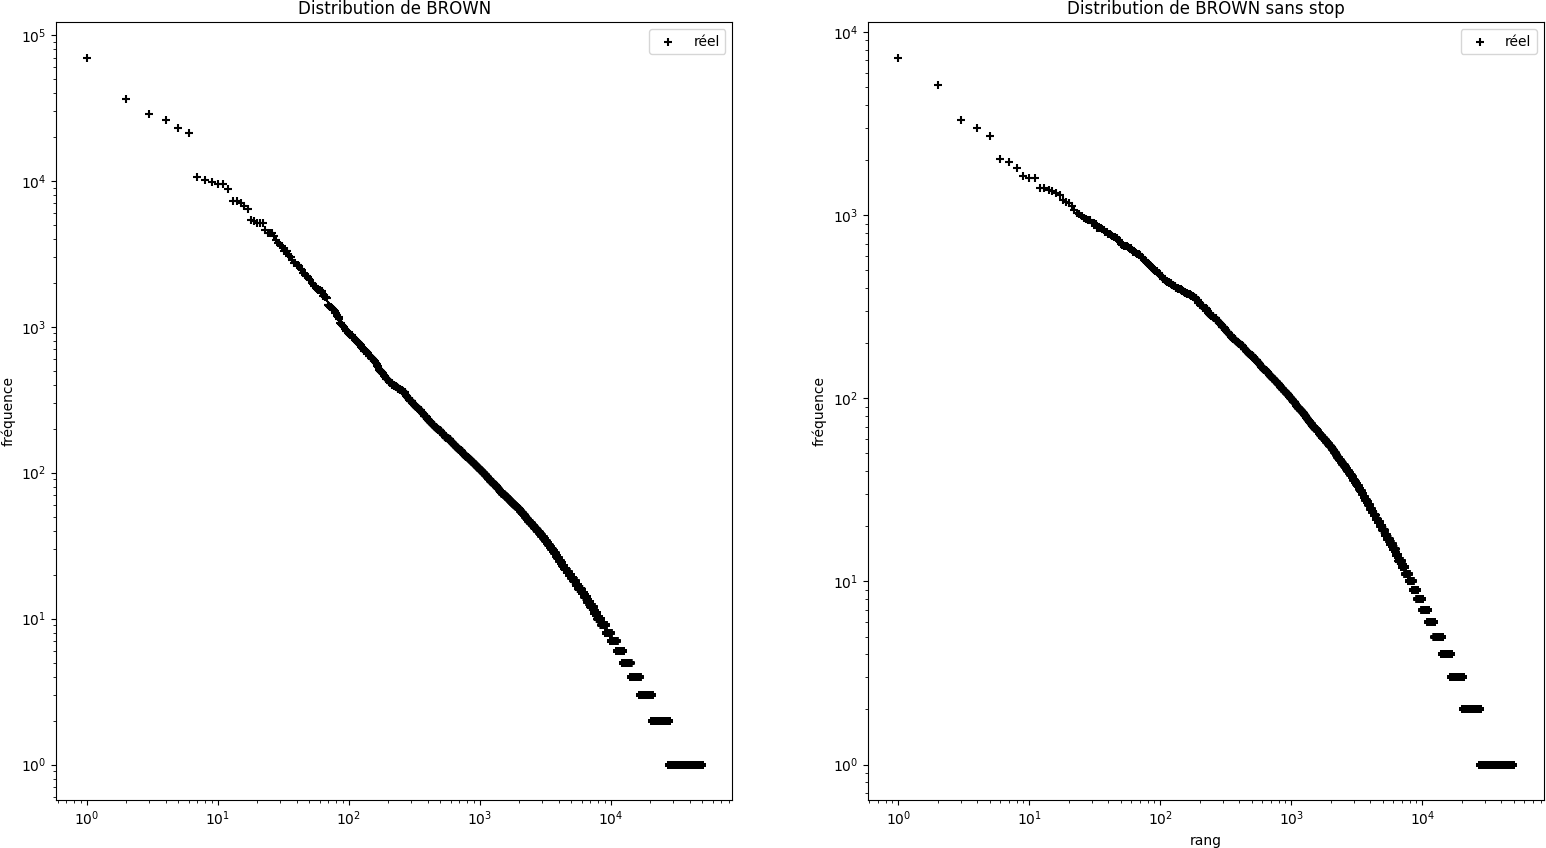
\includegraphics[width=\linewidth]{img/distribZipf.png}
				\caption{Distribution de Zipf pour les deux corpus}
		\end{figure}    		
    		
    		\begin{itemize}
    			\item Nombre de mots dans brown:	mots: 49398	occurences: 1012528
    			\item Nombre de mots dans brown stop:	mots: 49383	occurences: 578837\\
    		\end{itemize}
    		
    		La distribution de la version complète du corpus semble à première vue plus fidèle à la représentation classique de la distribution de Zipf. 
			
		\subparagraph{Etape 2 - calcul de la constante}
			Le premier paramètre qu'il faut déterminer est la \emph{constante}. Pour ce faire j'effectue le calcul suivant pour tous les mots :
			
			\begin{align*}
				constante = |mot| \times rang(mot)
			\end{align*}
			
			On obtient une liste de toutes les constantes théoriques pour chaque mot selon son rang.
			De cette liste, nous allons extraire la moyenne et la médiane.
			
			\begin{figure}[H]
				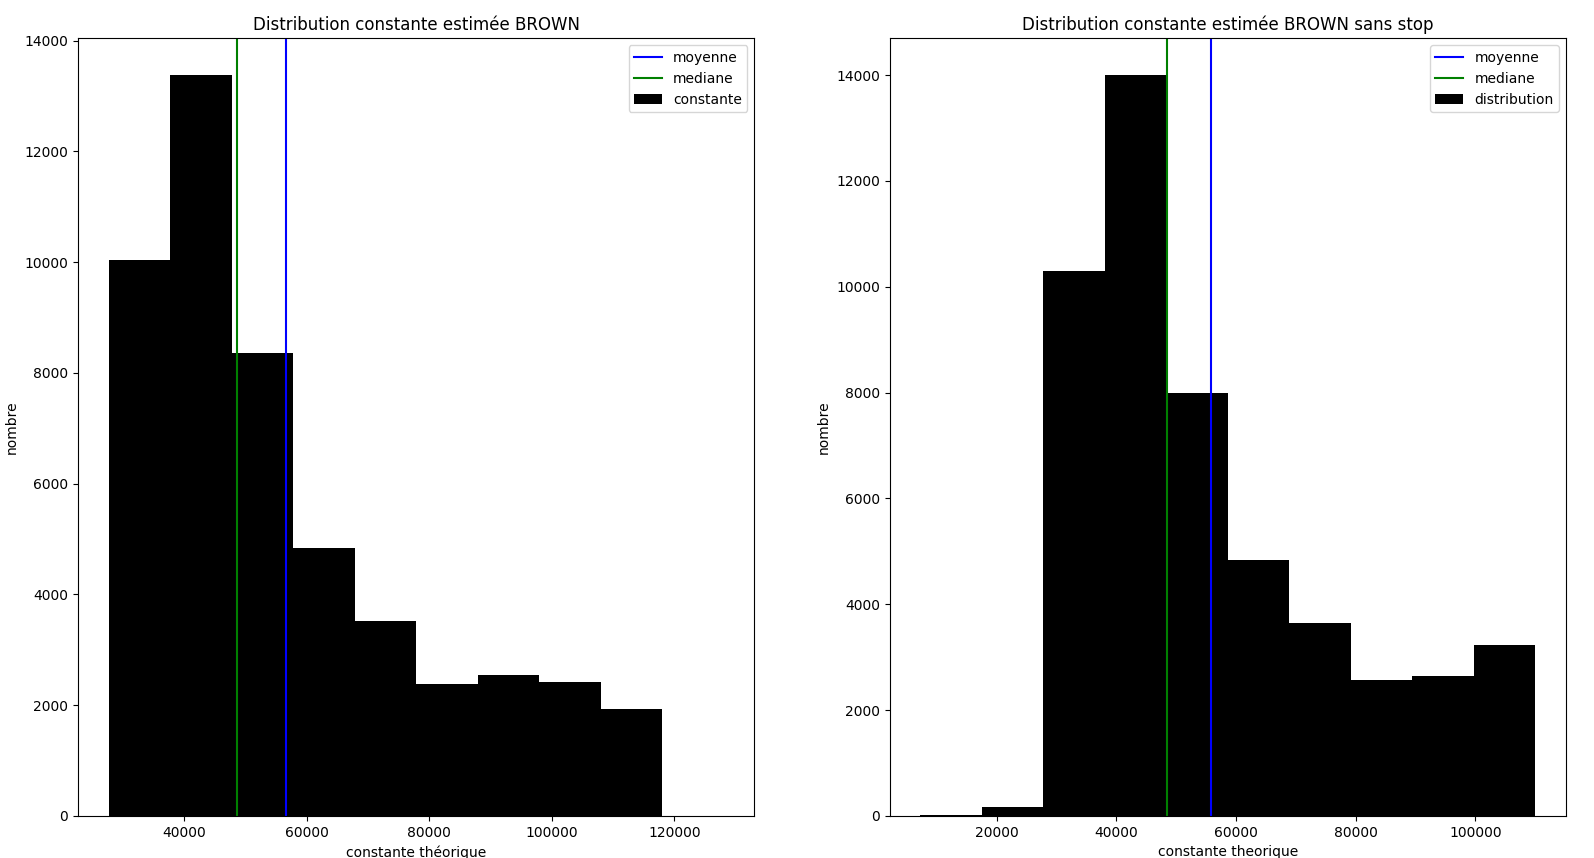
\includegraphics[width=\linewidth]{img/distribContTh.png}
				\caption{Distribution des constantes théoriques pour les deux corpus}
			\end{figure}
			
			On voit qu'il y a une majorité de mots donnant une constante brute comprise entre $20.000$ et $60.000$. Dans les deux corpus
			La différence entre les moyennes et médianes des deux corpus n'est pas flagrante :
			\begin{itemize}
				\item Brown moyenne: 56525.81, médiane: 48601.50
				\item Brown (- stopwords) moyenne: 55809.97, médiane: 48494.00
			\end{itemize}


		\subparagraph{Etape 3 - recherche du coefficient}
			Le coefficient $k$ permet d'ajuster le résultat, et pourra éventuellement donner une indication de complexité. La recherche de $k$ se fera sur les deux corpus avec utilisant les moyennes et médianes.\\
			
			Pour ce faire nous allons:

			\begin{enumerate}
				\item Faire la liste de tous les coefficients possibles dans l'intervalle $[0.86, 1.3]$ avec un pas de $0.01$\footnote{les bornes et le pas sont totalement arbitraire afin d'obtenir un graphique présentable}.
				\item Calculer toutes la fréquences théoriques de tous les rangs avec tous les coefficients possibles en utilisant les constantes moyenne et médiane de chaque corpus.
				\item Calculer la moyenne des coûts absolus entre les fréquences théoriques par coefficient avec la fréquence réelle observée pour chaque corpus.\\
			\end{enumerate}
			
			Le couple coefficient/constante avec le coup minimal sera retenu pour l'utilisation dans la phase de \emph{feature engineering}. \\	
			
			\begin{lstlisting}[title=Fonctions utilisées dans la recherche du coefficient]
def zipf_freq_theorique(constante, rang, coef):
    """
    Calcul la frequence theorique d'un mot selon son rang, la constante du texte et un coeficiant d'ajustement
    :param constante: <int> constante determinee par la distribution de Zipf
    :param rang: <int> rang du mot selon sa frequence
    :param coef: <float> variable d'ajustement
    :return: <float> frequence theorique zipfienne
    """
    return constante / (rang ** coef)
    
def cout(l1, l2, methode):
    """
    Calcul le cout de l'ecart entre les elements de l1 et le l2, place par place
    :param l1: <list> liste d'entier
    :param l2: <liste> liste d'entier
    :param methode: <str> methode de calcul du cout
    :return: <float> cout selon methode
    """
    if len(l1) != len(l2):
        print("Erreur, fonction cout: l1 & l2 de taille differente", file=sys.stderr)
        return None

    if len(l1) == 0:
        print("Erreur, fonction cout: liste vide", file=sys.stderr)

    if methode.lower() not in ['absolue', 'carre', 'racine']:
        print("Erreur, fonction cout - methode '{}' inconnue".format(methode), file=sys.stderr)
        return None

    if methode.lower() == 'absolue':
        return np.mean([abs(x-y) for x, y in zip(l1, l2)])

    if methode.lower() == 'carre':
        return np.mean([(x-y)**2 for x, y in zip(l1, l2)])

    if methode.lower() == 'racine':
        return np.sqrt(np.mean([(x-y)**2 for x, y in zip(l1, l2)]))

    return None\end{lstlisting}

			\begin{lstlisting}[title=Calcul des fréquences par coefficient]
    ls_coef = list(np.arange(0.86, 1.3, 0.01))
    zbmo_th = {coef: [stats.zipf_freq_theorique(zb_const_moyen, r, coef) for r in zb_rang] for coef in ls_coef}
    zbme_th = {coef: [stats.zipf_freq_theorique(zb_const_median, r, coef) for r in zb_rang] for coef in ls_coef}
    zbmoth_cmoy = [stats.cout(zb_freq, zbmo_th[coef], 'absolue') for coef in ls_coef]
    zbmeth_cmoy = [stats.cout(zb_freq, zbme_th[coef], 'absolue') for coef in ls_coef]

    zbsmo_th = {coef: [stats.zipf_freq_theorique(zbs_const_moyen, r, coef) for r in zbs_rang] for coef in ls_coef}
    zbsme_th = {coef: [stats.zipf_freq_theorique(zbs_const_median, r, coef) for r in zbs_rang] for coef in ls_coef}
    zbsmoth_cmoy = [stats.cout(zbs_freq, zbsmo_th[coef], 'absolue') for coef in ls_coef]
    zbsmeth_cmoy = [stats.cout(zbs_freq, zbsme_th[coef], 'absolue') for coef in ls_coef] \end{lstlisting}
		
		La recherche du coefficient nous retourne les éléments suivants:
			\begin{figure}[H]
				\includegraphics[width=\linewidth]{img/coutZipf.png}
				\caption{Coût absolu moyen par coefficient}
			\end{figure}
		
			\begin{itemize}
				\item Coût min brown moyenne: 5.93, median: 7.01
				\item Coût min brown (- stopwords) moyenne: 6.95, median: 6.46
				\item Coefficient min brown moyenne: 0.92, median: 0.91
				\item Coefficient min brown (- stopwords) moyenne: 0.97, median: 0.95
			\end{itemize}
				
	\paragraph{Résultats}
		
		Le tableaux ci dessous rappelle les données récupérées au long de la recherche:
		\begin{center}
			\begin{tabular}{|l|c|c|}
				\hline
				& BROWN avec stopwords & BROWN sans stopwords \\
				\hline
				nombre de mots uniques & 49398 & 49383 \\
				\hline
				nombre de mots total & 1012528 & 578837 \\
				\hline
				Constante moyenne & 56525.81 & 55809.97 \\
				\hline
				Constante médiane & 48601.50 & 48494.00 \\
				\hline
				Coefficient avec moyenne & 0.92 & 0.97 \\
				\hline
				Cout du coefficient moyenne & 5.93 & 6.95 \\
				\hline
				Coefficient avec médiane & 0.91 & 0.95 \\
				\hline
				Cout du coefficient médiane & 7.01  & 6.46 \\
				\hline
			\end{tabular}		
		\end{center}
		
		D'après les données il est possible de dire que l'on obtient de meilleurs résultats si on conserve tous les mots du corpus. Dans ce cas l'utilisation de la moyenne des constantes génère un taux d'erreur plus faible que la médiane.\\
		
		Ci-dessous la représentation des fréquences théoriques avec le coefficient optimal pour chaque corpus et chaque méthode. On voit que la courbe de la constante moyenne sur le corpus brute est celle qui suit le mieux les données réelles.
		\begin{figure}[H]
			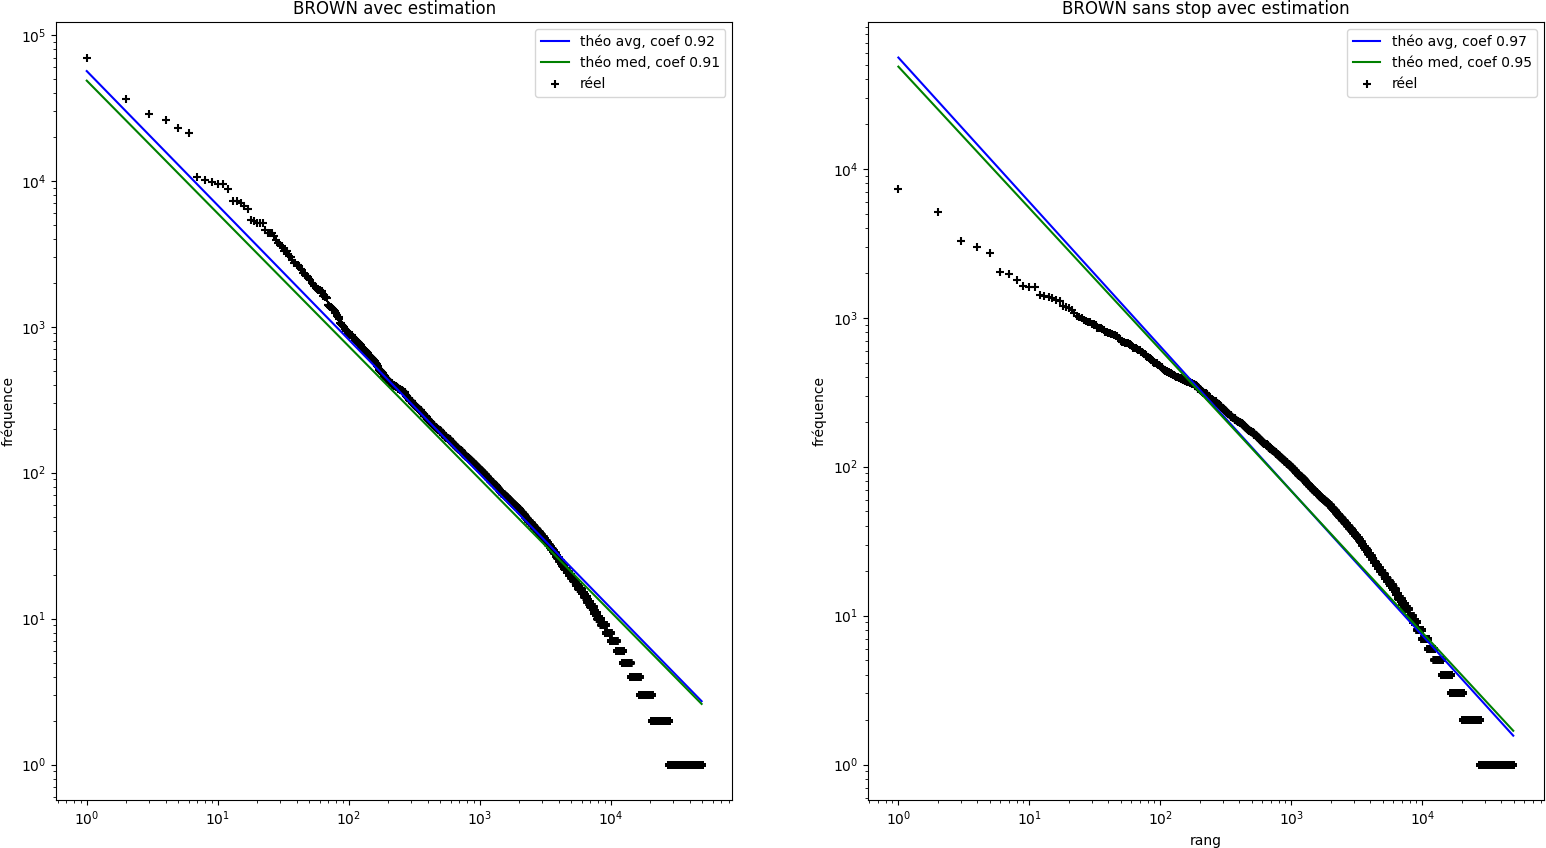
\includegraphics[width=\linewidth]{img/zipfFin.png}
			\caption{Distribution de Zipf avec les estimations}
		\end{figure}
		
		En conclusion, j'utiliserais la moyenne des constantes sur un document complet afin de déterminer le coefficient dans ma recherche de spam. 
		
		\subparagraph{Notes:}
			L'ensemble des codes sources pour cette partie est disponible dans les fichiers :
			\begin{itemize}
				\item[•]./analyse/rech\_zipf.py
				\item[•] ./traitement/stats.py
			\end{itemize}

\newpage
\section{Déploiement des bases de données}	
	Cette annexe détaille la mise en place de l'infrastructure de base de données pour le projet.
	J'utilise 2 environnements de base de données en version conteneur (docker version 23.0.4):
		\begin{itemize}
			\item ElasticSearch
				\begin{itemize}
					\item 1 Node Elastic, pour le service de base de données
					\item 1 Service Kibana, pour la visualisation des index
					\item 1 Service de certificat, pour sécuriser les échanges
				\end{itemize}
			\item PostgreSQL
				\begin{itemize}
					\item 1 service PostgreSQL, pour la base de données
					\item 1 service PgAdmin, pour la visualisation de la base
				\end{itemize}
		\end{itemize}
		
	Chaque environnement est indépendant, et possède une ouverture sur le PC hôte.
	
	
	\begin{figure}[H]
		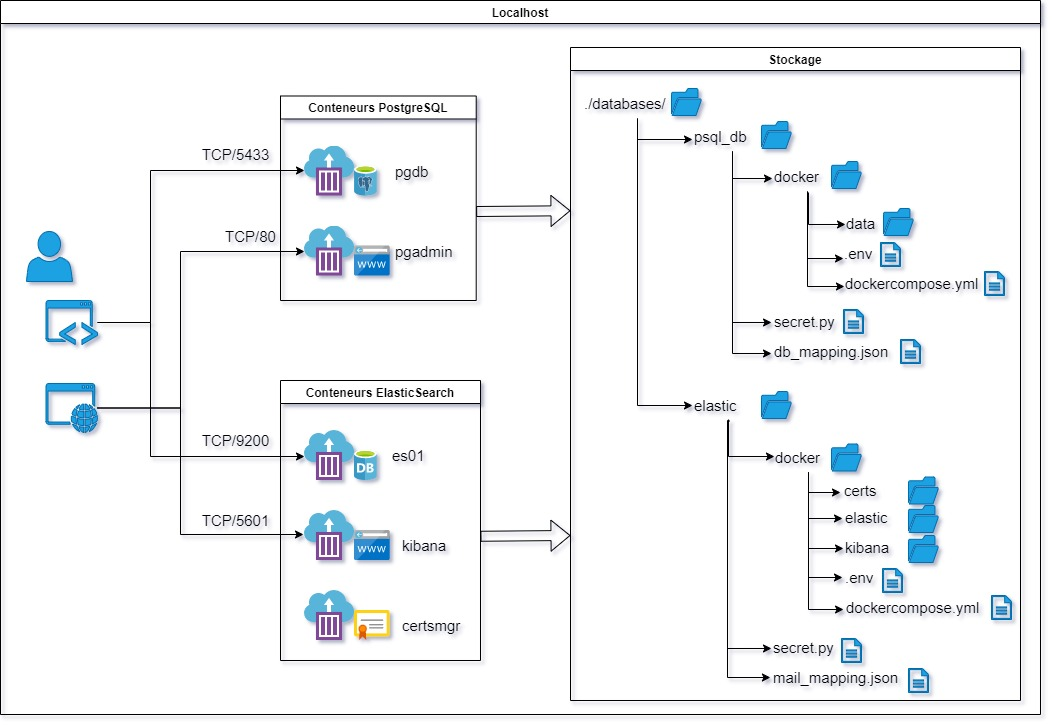
\includegraphics[width=\linewidth]{img/SchemaDocker.jpg}
		\caption{Schéma de l'architecture Docker}
	\end{figure}
	
	\subsection{ElasticSearch} \label{ES}
		Cet environnement se lance avec la commande suivante :
		\begin{verbatim}
docker compose -f ./databases/elastic/docker/docker-compose.yml up -d		
		\end{verbatim}
		
		\subsubsection{Conteneurisation}
			\begin{lstlisting}[title=DockerCompose]
version: "3.2"

services:
        certsmgr:
                image: elasticsearch:${VERSION}
                volumes:
                        - ./certs:/usr/share/elasticsearch/config/certs
                user: "0"
                command: >
                        bash -c '
                                if [ x${ELASTIC_PASSWORD} == x ]; then
                                        echo "Set the ELASTIC_PASSWORD environment variable in the .env file";
                                        exit 1;
                                elif [ x${KIBANA_PASSWORD} == x ]; then
                                        echo "Set the KIBANA_PASSWORD environment variable in the .env file";
                                        exit 1;
                                fi;
                                if [ ! -f certs/ca.zip ]; then
                                        echo "Creating CA";
                                        bin/elasticsearch-certutil ca --silent --pem -out config/certs/ca.zip;
                                        unzip config/certs/ca.zip -d config/certs;
                                fi;
                                if [ ! -f certs/certs.zip ]; then
                                        echo "Creating certs";
                                        echo -ne \
                                                "instances:\n"\
                                                "  - name: es01\n"\
                                                "    dns:\n"\
                                                "      - es01\n"\
                                                "      - localhost\n"\
                                                "    ip:\n"\
                                                "      - 127.0.0.1\n"\
                                                > config/certs/instances.yml;
                                        bin/elasticsearch-certutil cert --silent --pem -out config/certs/certs.zip --in config/certs/instances.yml --ca-cert config/certs/ca/ca.crt --ca-key config/certs/ca/ca.key;
                                        unzip config/certs/certs.zip -d config/certs;
                                fi;
                                # echo "Setting file permissions"
                                echo "chown -R root:root config/certs";
                                echo "find . -type d -exec chmod 750 \{\} \;";
                                echo "find . -type f -exec chmod 640 \{\} \;";
                                echo "Waiting for Elasticsearch availability";
                                until curl -s --cacert config/certs/ca/ca.crt https://es01:9200 | grep -q "missing authentication credentials"; do sleep 30; done;
                                echo "Setting kibana_system password";
                                until curl -s -X POST --cacert config/certs/ca/ca.crt -u elastic:${ELASTIC_PASSWORD} -H "Content-Type: application/json" https://es01:9200/_security/user/kibana_system/_password -d "{\"password\":\"${KIBANA_PASSWORD}\"}" | grep -q "^{}"; do sleep 10; done;
                                echo "All done!";
                        '
                healthcheck:
                        test: ["CMD-SHELL", "[ -f config/certs/es01/es01.crt ]"]
                        interval: 1s
                        timeout: 5s
                        retries: 120


        es01:
                depends_on:
                        certsmgr:
                                condition: service_healthy
                image: elasticsearch:${VERSION}
                volumes:
                        - ./certs:/usr/share/elasticsearch/config/certs
                        - ./elastic/data:/usr/share/elasticsearch/data
                ports:
                        - ${ES_PORT}:9200
                environment:
                        - discovery.type=single-node
                        - ELASTIC_PASSWORD=${ELASTIC_PASSWORD}
                        - bootstrap.memory_lock=true
                        - xpack.security.enabled=true
                        - xpack.security.http.ssl.enabled=true
                        - xpack.security.http.ssl.key=certs/es01/es01.key
                        - xpack.security.http.ssl.certificate=certs/es01/es01.crt
                        - xpack.security.http.ssl.certificate_authorities=certs/ca/ca.crt
                        - xpack.security.http.ssl.verification_mode=certificate
                        - xpack.security.transport.ssl.enabled=true
                        - xpack.security.transport.ssl.key=certs/es01/es01.key
                        - xpack.security.transport.ssl.certificate=certs/es01/es01.crt
                        - xpack.security.transport.ssl.certificate_authorities=certs/ca/ca.crt
                        - xpack.security.transport.ssl.verification_mode=certificate
                        - xpack.license.self_generated.type=${LICENSE}
                mem_limit: ${MEM_LIMIT}
                ulimits:
                        memlock:
                                soft: -1
                                hard: -1
                healthcheck:
                        test:
                                [
                                        "CMD-SHELL",
                                        "curl -s --cacert config/certs/ca/ca.crt https://localhost:9200 | grep -q 'missing authentication credentials'",
                                ]
                        interval: 10s
                        timeout: 10s
                        retries: 120

        kibana:
                depends_on:
                        es01:
                                condition: service_healthy
                image: kibana:${VERSION}
                volumes:
                - ./certs:/usr/share/kibana/config/certs
                - ./kibana/data:/usr/share/kibana/data
                ports:
                - ${KIBANA_PORT}:5601
                environment:
                        - SERVERNAME=kibana
                        - ELASTICSEARCH_HOSTS=https://es01:9200
                        - ELASTICSEARCH_USERNAME=kibana_system
                        - ELASTICSEARCH_PASSWORD=${KIBANA_PASSWORD}
                        - ELASTICSEARCH_SSL_CERTIFICATEAUTHORITIES=config/certs/ca/ca.crt
                mem_limit: ${MEM_LIMIT}
                healthcheck:
                        test:
                                [
                                        "CMD-SHELL",
                                        "curl -s -I http://localhost:5601 | grep -q 'HTTP/1.1 302 Found'",
                                ]
                        interval: 10s
                        timeout: 10s
                        retries: 120
			\end{lstlisting}
			
			\begin{lstlisting}[title=Fichier d'environnement]
# Password for elastic user
ELASTIC_PASSWORD=XXXXXXXXX
# Password for kibana_system user
KIBANA_PASSWORD=XXXXXXXXX
# Version elastic product
VERSION=8.1.2
# Licence to use
LICENSE=basic
# Port for elastic HTTP API
ES_PORT=9200
#ES_PORT=127.0.0.1:9200
# Port for kibana access
KIBANA_PORT=5601
# Memory available (bytes)
MEM_LIMIT=322122547
			\end{lstlisting}

		\subsubsection{Initialisation de l'index}
		
			\begin{lstlisting}[title=Exemples de secrets]
serveur = "https://localhost:9200"
apiid = "XXXXXXXXXXXXXXXXXXXXXXX"
apikey = "XXXXXXXXXXXXXXXXXXXXXX"
ca_cert = "databases/elastic/docker/certs/ca/ca.crt"
			\end{lstlisting}
			Il est possible de générer une clé API via l'interface Kibana > Stack Management > Sécurité > API keys > Create API Key > JSON. 
			
			\begin{lstlisting}[title=Mapping de l'index]
{
  "properties": {
    "hash": {"type": "keyword"},
    "categorie": {"type": "keyword"},
    "sujet": {"type": "text"},
    "expediteur": {"type": "text"},
    "message": {"type": "text"},
    "langue": {"type": "keyword"}
  }
}
			\end{lstlisting}
			
			
				\begin{lstlisting}[title=Fonctions Python utiles]
def es_connect(server, creds, crt):
    """ Connexion au serveur ElasticSearch """
    client = Elasticsearch(server, api_key=creds, ca_certs=crt)

    try:
        client.search()
        client.indices.get(index="*")
        return client

    except (exceptions.ConnectionError, AuthenticationException, AuthorizationException) as err:
        print("ES:conn - Informations client ElasticSearch :\n\t", err)
        client.close()
        return None


def es_create_indice(es_cli, index, mapping):
    """ Creer un indice s'il n'existe pas deja """
    indices = es_cli.indices.get(index='*')
    if indices and index in indices:
        print("Warning: Indice {} deja present".format(index), end=' ')
        return

    try:
        res = es_cli.indices.create(index=index, mappings=mapping)
    except elasticsearch.ApiError as err:
        print(err)
        return

    if not res['acknowledged']:
        print("Error : Echec de la creation de l'indice {}".format(index))
				\end{lstlisting}
				


	\subsection{PostgreSQL} \label{PSQL}
		Cet environnement se lance avec la commande suivante :
		\begin{verbatim}
docker compose -f ./databases/psql_db/docker/docker-compose.yml up -d		
		\end{verbatim}
		
		Le programme se charge automatiquement de créer le compte utilisé pour se connecter à la base.
				
		\subsubsection{Conteneurisation}
			\begin{lstlisting}[title=DockerCompose]
version: "3.3"
services:
        pgdb:
                image: postgres:${PS_VERSION}
                restart: always
                environment:
                        POSTGRES_PASSWORD: ${PS_PASSWORD}

                volumes:
                        - ./data:/var/lib/postgresql/data
                ports:
                        - ${PS_PORT}:5432

        pgadmin:
                image: dpage/pgadmin4:${PS_VERSION}
                environment:
                        PGADMIN_DEFAULT_EMAIL: ${PGA_MAIL}
                        PGADMIN_DEFAULT_PASSWORD: ${PGA_PASSWORD}
                ports:
                        - ${PGA_PORT}:80
                depends_on:
                        - pgdb
			\end{lstlisting}
			
			\begin{lstlisting}[title=Fichier d'environnement]
PS_VERSION=latest

PS_PASSWORD=XXXXXXXXX
PS_PORT=5433

PGA_MAIL=data@data.org
PGA_PASSWORD=XXXXXX
PGA_PORT=80
			\end{lstlisting}

		\subsubsection{Initialisation de la base de données}
		
			\begin{lstlisting}[title=Exemples de secrets.py]
owner = "XXX"
owner_pw = "XXX"
admin = "XXXX"
admin_pw = "XXXX"
host = "localhost"
port = "5432"
			\end{lstlisting}
			
			\begin{lstlisting}[title=Mapping]
{
  "mail_features": {
    "categories": {
      "id_cat": ["SERIAL", "PRIMARY KEY"],
      "type": ["VARCHAR", "UNIQUE", "NOT NULL"]
    },
    "messages": {
      "id_message": ["SERIAL", "PRIMARY KEY"],
      "hash": ["CHAR(32)", "UNIQUE", "NOT NULL"],
      "id_cat": ["INT", "NOT NULL"],
      "fk": ["fk_message", "id_cat", "categories(id_cat)", "SET NULL"]
    },
    "liens": {
      "id_message": ["INT"],
      "url": ["INT"],
      "mail": ["INT"],
      "tel": ["INT"],
      "nombre": ["INT"],
      "prix": ["INT"],
      "fk": ["fk_liens", "id_message", "messages(id_message)", "CASCADE"]
    },
    "stats_mots": {
      "id_message": ["INT"],
      "mots_uniques": ["INT"],
      "mots": ["INT"],
      "char": ["INT"],
      "char_maj": ["INT"],
      "mot_maj": ["INT"],
      "mot_cap": ["INT"],
      "fk": ["fk_stats_mot", "id_message", "messages(id_message)", "CASCADE"]
    },
    "stat_ponct": {
      "id_message": ["INT"],
      "point": ["INT"],
      "virgule": ["INT"],
      "exclamation": ["INT"],
      "interrogation": ["INT"],
      "espace": ["INT"],
      "tabulation": ["INT"],
      "ligne": ["INT"],
      "ligne_vide": ["INT"],
      "fk": ["fk_stats_ponct", "id_message", "messages(id_message)", "CASCADE"]
    },
    "zipf": {
      "id_message": ["INT"],
      "constante": ["INT"],
      "coefficient": ["REAL"],
      "tx_erreur": ["REAL"],
      "fk": ["fk_zipf", "id_message", "messages(id_message)", "CASCADE"]
    },
    "hapax": {
      "id_message": ["INT"],
      "ratio_unique": ["REAL"],
      "ratio_texte": ["REAL"],
      "fk": ["fk_hapax", "id_message", "messages(id_message)", "CASCADE"]
    }
  }
}
			\end{lstlisting}
			
			\begin{lstlisting}[title=Fonctions utiles]
def create_db(nom, owner, user, passwd, host, port):
    """ Creer une nouvelle base de donnees """
    client_psql = psycopg2.connect(user=user, password=passwd, host=host, port=port)
    client_psql.autocommit = True
    cursor = client_psql.cursor()

    cursor.execute("DROP DATABASE IF EXISTS {};".format(nom))
    cursor.execute("CREATE DATABASE {};".format(nom))
    cursor.execute("ALTER DATABASE {} OWNER TO {};".format(nom, owner))
    client_psql.close()


def connect_db(database, user, passwd, host, port):
    """ Connexion a la base de donnees Postgres. Penser a fermer la connexion """
    try:
        client_psql = psycopg2.connect(database=database, user=user, password=passwd, host=host, port=port)
    except psycopg2.Error as e:
        print("Erreur de connexion : \n{}".format(e), file=sys.stderr)
        return None

    client_psql.autocommit = True
    return client_psql


def create_table(client_psql, nom, champs):
    """ Creer une nouvelle table dans la base de donnees """
    fk = ""
    fields = []

    curseur = client_psql.cursor()
    curseur.execute(f"DROP TABLE IF EXISTS {nom}")

    if 'fk' in champs.keys():
        ls = champs.pop('fk')
        fk = f"CONSTRAINT {ls.pop(0)} FOREIGN KEY({ls.pop(0)}) REFERENCES {ls.pop(0)}"
        if ls:
            fk += f" ON DELETE {ls.pop(0)}"

    for key, value in champs.items():
        fields.append(f"{key} {' '.join(value)}")

    query = f"CREATE TABLE {nom} ({', '.join(fields)})"
    if fk:
        query = query[:-1] + f", {fk})"
    curseur.execute(query)


def create_index(client_psql, nom, table, colonne):
    """ Index sur une colonne """
    query = "CREATE UNIQUE INDEX {} ON {}({})".format(nom, table, colonne)
    exec_query(client_psql, query)
			\end{lstlisting}
				

\newpage
\section{Tableau des choix technologiques}
	\begin{tabular}{|p{3cm}|c|p{4cm}|p{6cm}|}
		\hline
		Élément & Retenu & Raisons & Observations \\
		\hline
		
		\multicolumn{4}{|c|}{Datasets} \\
		\hline
		Mail de la compagnie Enron & Non & Mails non classés & Non retenu pour la phase de développement car pas de moyen fiable de contrôler la sortie automatiquement \\
		\hline
		Mail du projet SpamAssassin & Oui & Mails déjà pré-triés & Mails principalement en Anglais déjà pré-trié en catégorie Spam et Ham \\
		\hline
		Brown dataset (nltk) & Oui & Corpus d'un million de mots en Anglais publié en 1961 & Dataset utilisé pour le développement de la visualisation de la distribution de Zipf\\
		\hline
		Stopwords (nltk) & Oui & Corpus de mots commun non significatif dans un texte & Utilisation dans le développement de la visualisation de la distribution de Zipf\\
		\hline
		
		\multicolumn{4}{|c|}{Langage et Modules} \\
		\hline
		Python & Oui & Langage polyvalent pour le traitement des données & \\		
		\hline
		Module email & Oui & Module natif pour le traitement des mails & Grande flexibilité pour la lecture des mails \\
		\hline
		
		\multicolumn{4}{|c|}{Virtualisation} \\
		\hline
		Docket & Oui & configuration et environnement dans les fichiers. Cela facilite le portage vers d'autre environnement & Lors du développement j'ai pu utilisé mon PC personnel sous Linux et un autre PC sous Windows. L'utilisation de Docker m'a évité de nombres configurations sur Windows\\
		\hline
		
		\multicolumn{4}{|c|}{Bases de données} \\
		\hline
		ElasticSearch & Oui & Technologie utilisée dans mon entreprise. Présence d'une interface de visualisation des données Kibana. & Application dockerisée. \\
		\hline
		PostgreSQL & Oui & Moteur de base de données relationnelle plus facilement scalable que ElasticSearch pour l'ajout de nouvelle catégorie de données. Il n'est pas nécessaire de ré-indexer toute la base pour ajouter des champs & Application dockerisée\\
		\hline
		SQLite & Oui & Base de données légère pour stocker uniquement les données statistiques des étapes de la phase 1 & Rapide à mettre en place et déjà intégrée \\
		\hline		
		
		\hline
	\end{tabular}
	
	\section{Modèles}	
		\subsection{Naïves Bayes}
			Ce type de modèle est utilisé par le module \emph{langdetect} qui me sert pour la détection des langues.
			
			\paragraph{Introduction}
				Les modèles Naïves Bayes se basent sur le théorème de probabilité de Bayes. Il permet de déterminer la probabilité conditionnelle d'apparition d'un évènement A sachant qu'un évènement B s'est produit. Le terme naïf fait référence au fait que l'on présuppose que les évènements A et B ne sont pas corrélés.\\
				Ces techniques sont utilisées pour des modèles de classification en apprentissage supervisé.\\
				
				La formule mathématique de ce théorème est la suivante :
				\begin{eqnarray}\label{NBeq}
					P(A|B) &=& \frac{P(B|A)P(A)}{P(B)}
				\end{eqnarray}
				
			On recherche ici $P(A|B)$, c'est a dire la probabilité d'apparition d'un évènement A sachant que l'évènement B s'est produit. \\ 
			
			Pour ce faire nous avons besoin des données suivantes :
			\begin{itemize}
				\item $P(B|A)$ est la probabilité que l'évènement B s'est produit sachant que l'évènement A s'est produit
				\item $P(A)$ est la probabilité d'apparition de l'évènement A
				\item $P(B)$ est la probabilité d'apparition de l'évènement B
			\end{itemize}
			
			\paragraph{Exemples d'utilisation}
				Les exemples ci dessous vont permettre d'illustrer l'utilisation de cette technique. D'abord manuellement sur un petit jeu de données puis à l'aide d'un code pré-existant sur un autre jeu de données plus important.
				
				\subparagraph{Manuel}
					Dans cet exemple nous allons déterminer la probabilité qu'a un joueur d'aller sur le terrain selon les conditions météorologiques. Cette probabilité sera calculée en fonction des données récupérées lors des matchs précédents.\footnote{Les données présentées sont inventées} \\
					
					On recherchera ainsi la probabilité de présence sur le terrain d'un joueur selon la météo $P(A|B)$. Pour ce faire nous auront besoin de: 
					\begin{itemize}
						\item $P(A)$ Probabilité de jouer quelque soit le temps
						\item $P(B)$ Probabilité de l'évènement météorologique
						\item $P(B|A)$ Probabilité de l'évènement sachant que le joueur a été sur le terrain					
					\end{itemize}
				
				\begin{table}[H]
					\centering
					\captionof{table}{Données de présence sur le terrain} \label{tab:data}
					\begin{tabular}{|l|c|c|c|c|c|c|c|}
						\hline
						météo & soleil & soleil & couvert & pluie & pluie & pluie & couvert \\
						\hline
						présent & non & non & oui & oui & oui & non & oui \\
						\hline
						\hline
						météo & soleil & soleil & pluie & soleil & couvert & couvert & pluie \\
						\hline
						présent & non & oui & oui & oui & oui & oui & non \\
						\hline
					\end{tabular}
				\end{table}
				
				\begin{table}[H]
					\centering
					\captionof{table}{Synthèse et probabilité simple P(A) et P(B)} \label{tab:pab}
					\begin{tabular}{|l|c|c|r|}
						\hline
						météo & oui & non & $P(B)$\\
						\hline
						couvert & 4 & 0 & $4/14$\\
						\hline
						soleil & 2 & 3 & $5/14$\\
						\hline
						pluie & 3 & 2 & $5/14$\\
						\hline
						$P(A)$ & $9/14$ & $5/14$ & \\
						\hline
					\end{tabular}
				\end{table}
						
				On peut déterminer les probabilités de chaque météo en fonction de la présence du joueur sur le terrain P(B|A). Pour ce faire on divise le nombre d'évènements de présence du joueur lors d'un évènement météo par le nombre total d'évènements de présence du joueur
				
				\begin{table}[H]
					\centering
					\captionof{table}{Probabilité météo selon présence du joueur} \label{tab:pba}
					\begin{tabular}{|l|c|c|}
						\hline
						météo & P(B|oui) & P(B|non) \\
						\hline
						couvert & $4/9$ & $0/5$ \\
						\hline
						soleil & $2/9$ & $3/5$ \\
						\hline
						pluie & $3/9$ & $2/5$ \\
						\hline	
					\end{tabular}
				\end{table}
				
				On va maintenant calculer la probabilité qu'à un joueur d'être sur le terrain si le temps est couvert.\\
				On commence par la probabilité du oui:
				\begin{eqnarray*}
					P(A|B) &=& \frac{P(B|A)P(A)}{P(B)}\\
					P(A|B) &=& \frac{\frac{4}{9}\cdot\frac{9}{14}}{\frac{4}{14}}\\
					P(A|B) &=& \frac{\frac{4}{14}}{\frac{4}{14}}\\
					P(A|B) &=& \frac{4}{14}\cdot\frac{14}{4}\\
					P(A|B) &=& 1
				\end{eqnarray*}
				
				On enchaîne sur la probabilité de ne pas jouer si le temps est couvert
				\begin{eqnarray*}
					P(A|B) &=& \frac{P(B|A)P(A)}{P(B)}\\
					P(A|B) &=& \frac{\frac{0}{5}\cdot\frac{5}{14}}{\frac{4}{14}}\\
					P(A|B) &=& 0\cdot\frac{14}{4}\\
					P(A|B) &=& 0
				\end{eqnarray*}	
				
				On peut dire que si le temps est couvert le joueur très probablement sur le terrain			 
				On peut également déterminer la probabilité de jouer pour chaque évènement météo
				\begin{table}[H]
					\centering
					\captionof{table}{Probabilité présence du joueur selon la météo} \label{tab:pab2}
					\begin{tabular}{|l|c|c|c|}
						\hline
						météo & oui & non & plus probable\\
						\hline
						couvert & 1 & 0 & oui\\
						\hline
						soleil & 2/5 & 3/5 & non \\
						\hline
						pluie & 3/5 & 2/5 & oui \\
						\hline
					\end{tabular}
				\end{table}
				
				\emph{Cas polynomial}: Il est possible de déterminer la probabilité d'un évènement par rapport à plus autres. Dans ce cas, il faudra multiplier entre elles les probabilités de ces évènements selon l'apparition de l'évènement voulu.\\
				
				 Calcul pour un évènement (A) selon 2 autres évènements (B et C)
				 \begin{eqnarray*}
				 	P(A|BC) &=& \frac{P(B|A)P(C|A)P(A)}{P(B)P(C)}
				 \end{eqnarray*}
				
				\subparagraph{En code} Dans cet exemple nous allons utiliser un code existant dans la librairie python scikit-learn\cite{scikit-learn}. Ce moteur Naïves Bayes va nous permettre cette fois-ci de catégoriser des variétés d'iris selon la longueur et la largeur des pétales et des sépales. Les données proviennent cette fois-ci d'un dataset également disponible dans scikit-learn.
				
				Nous allons utilisé le modèle \emph{GaussianNB} de scikit-learn qui est adapté lorsque les données utilisées suivent une distribution normale. Ce qui semble être le cas pour les longueurs et largeur des sépale. 
				\begin{figure}[H]
					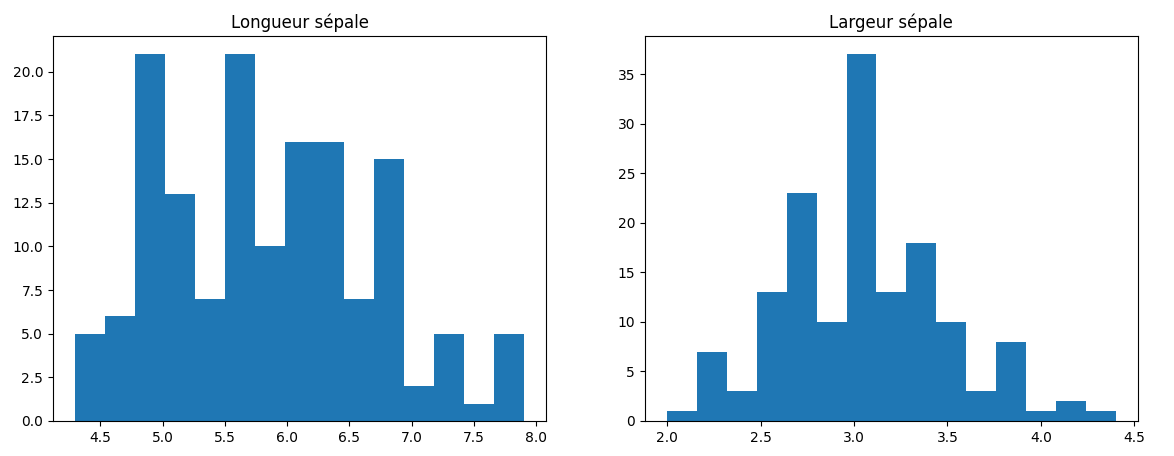
\includegraphics[width=\linewidth]{img/NBdistrib.png}
					\caption{Distribution des longueurs et largeurs des sépales}
				\end{figure}
				
\begin{lstlisting}[title=Progamme complet]
from sklearn.datasets import load_iris
from sklearn.model_selection import train_test_split
from sklearn.naive_bayes import GaussianNB
from sklearn.metrics import accuracy_score, confusion_matrix, ConfusionMatrixDisplay, f1_score, \
    recall_score

import matplotlib.pyplot as plt

X, y = load_iris(return_X_y=True)

X_train, X_test, y_train, y_test = train_test_split(X, y, test_size=0.33, random_state=0)
model = GaussianNB()
model.fit(X_train, y_train)

y_pred = model.predict(X_test)
precision = accuracy_score(y_pred, y_test)
recall = recall_score(y_test, y_pred, average="weighted")
f1 = f1_score(y_pred, y_test, average="weighted")

print("Precision:", precision)
print("Rappel:", recall)
print("Score F1:", f1)

plt.figure('Donnees du modele', figsize=(14, 5))
plt.subplot(1, 3, 1, title='Donnees du train set')
plt.scatter(X_train[:, 0], X_train[:, 1], c=y_train)
plt.xlabel('Sepale long.')
plt.ylabel('Sepale larg.')
plt.subplot(1, 3, 2, title='Donnees du test set')
plt.scatter(X_test[:, 0], X_test[:, 1], c=y_test)
plt.xlabel('Sepale long.')
plt.subplot(1, 3, 3, title='Donnees test apres evaluation')
plt.scatter(X_test[:, 0], X_test[:, 1], c=y_pred)
plt.xlabel('Sepale long.')
plt.show()

cm = confusion_matrix(y_test, y_pred, labels=[0, 1, 2])
disp = ConfusionMatrixDisplay(confusion_matrix=cm, display_labels=[0, 1, 2])
disp.ax_.set_title('Matrice de confusion')
disp.plot()
plt.show()

plt.figure('Distribution des donnees Iris', figsize=(14, 5))
plt.subplot(1, 2, 1, title='Longueur sepale')
plt.hist(X[:, 0], bins=15)
plt.subplot(1, 2, 2, title='Largeur sepale')
plt.hist(X[:, 1], bins=15)
plt.show()\end{lstlisting}
				
				Les données du dataset ont été séparés en 2 jeux, un pour l’entraînement du modèle et un pour le test. On obtient alors la représentation suivantes après entrainement et test du modèle
				\begin{figure}[H]
					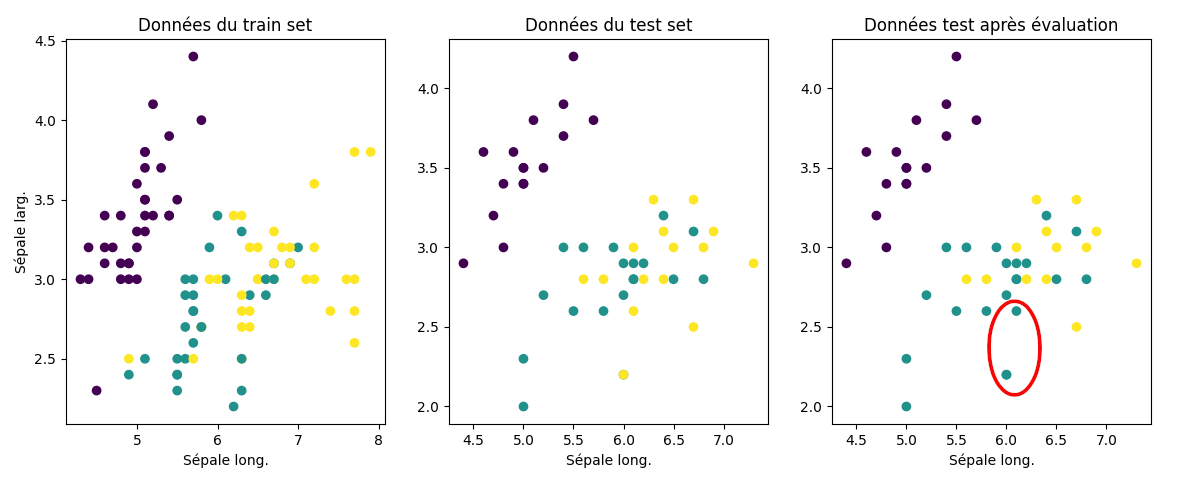
\includegraphics[width=\linewidth]{img/NBdata.png}
					\caption{Représentation des données }
				\end{figure}
				
				Dans les données de test nous avons 2 catégorisations qui n'ont pas été réalisées correctement. On obtient les scores suivants :
				\begin{itemize}
					\item Précision: 0.96                    \footnote{La précision est la proportion des éléments correctement identifiés sur l'ensemble des éléments prédit}
					\item Rappel: 0.96						\footnote{Le rappel est la proportion des éléments correctement identifiés sur l'ensemble des éléments de la catégorie}
					\item Score F1: 0.9604285714285714		\footnote{Le Score F1 est la moyenne harmonique calculée de la manière suivante $2*(precision*rappel)/(precision+rappel)$}
				\end{itemize}				
				
				\begin{figure}[H]
					\centering
					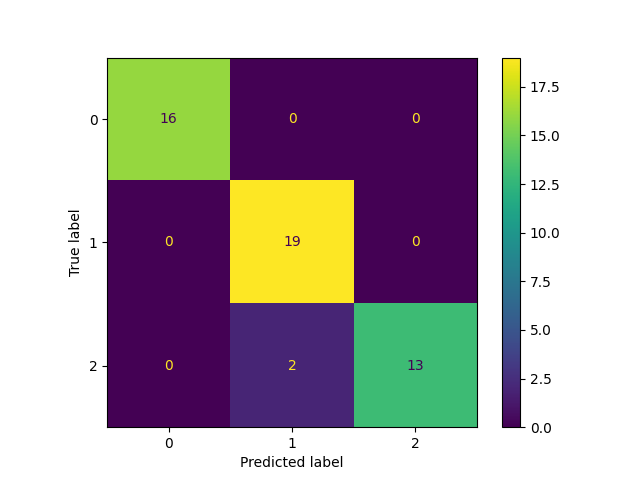
\includegraphics[scale=0.7]{img/NBmatrix.png}
					\caption{Matrice de confusion}
				\end{figure}
				
				A l'aide de ce modèle nous devrions avoir une 96\% de chance de déterminer la bonne variété d'iris en se basant sur la longueur et la largeur des sépales.  
				
			\paragraph{Avantages et inconvénients} 
				Le modèle Naïve Bayes est un modèle simple et rapide qui ne nécessite pas de grande capacités de calcul. De ce fait il permet de traiter une grande quantité de données.\\
				
				Cependant, les données qui lui sont fournies ne doivent pas être corrélées ce qui est rarement le cas dans les problèmes du monde réel. Ce type de modèle est limité à des problèmes de classification supervisée. Si on se fie à l'équation (\ref{NBeq}) la probabilité d'apparition de l’évènement B : P(B) ne peut pas être nulle. 
				
										
	\section{Bibliographie}
		\bibliographystyle{plain}
		\bibliography{IED_L3_Projet_Inglang_Fouille_IA}
		


		
	\section{Sitotec}
		\subsection{Corpus}
			\begin{itemize}
				\item Enron company mails, fichier CSV contenant l'ensemble des mails d'une entreprise ayant fermée ses portes (33.834.245 mails) [en ligne], \url{https://www.kaggle.com/wcukierski/enron-email-dataset} (consulté le 27/01/2022) \label{Enron_dataset}
				\item Mails project SpamAssassin, projet opensource de détection de spam (6065 fichiers email déjà trier en ham et spam) [en ligne], \url{https://spamassassin.apache.org/old/publiccorpus/} (consulté le 27/01/2022) \label{SpamAssassin_dataset}
				\item Brown corpus, ensemble de texte en anglais publié en 1961 qui contient plus d'un million de mots \url{https://www.nltk.org/book/ch02.html} (consulté le 20/08/2022) \label{Brown_corpus}
			\end{itemize}
		
		\subsection{Modules}
			\paragraph{Module langdetect}
			\begin{itemize}
				\item Page Github du projet \emph{langdetect} capable de différencier 49 langages avec une précision de 99\%, [en ligne] \url{https://github.com/Mimino666/langdetect} (consulté le 04/12/2022) \label{langdetect}
				\item Language Detection Library, présentation du module (anglais) [en ligne] \url{https://www.slideshare.net/shuyo/language-detection-library-for-java} (consulté le 04/12/2022)
			\end{itemize}
			
		\subsection{Modèles}
			\paragraph{Naïves Bayes}
				Le modèle Naïves Bayes est employé dans le module langdetect (\ref{langdetect})
			\begin{itemize}
				\item Les algorithmes de Naïves Bayes, Explication sommaire du principe de ces type d'algorithme, [en ligne] \url{https://brightcape.co/les-algorithmes-de-naives-bayes/} (consulté le 26/03/2023)
				\item Naive Bayes Classification Tutorial using Scikit-learn, exemple d'utilisation de ce type de modèle avec python (anglais) [en ligne] \url{https://www.datacamp.com/tutorial/naive-bayes-scikit-learn} (consulté le 26/03/2023)
				\item Scikit learn Naive Bayes, description des types d'algorithme disponibles dans le module Scikitlearn en python (anglais) [en ligne] \url{https://scikit-learn.org/stable/modules/naive_bayes.html} (consulté le 26/03/2023)
			\end{itemize}
			
	\section{Codes sources}
		\subsection{Github}
			Le lien vers l'ensemble des sources est disponible en publique via le lien ci dessous:\\
			\url{https://github.com/peredur0/mercury}
			
		\subsection{Analyse statistiques de la phase 1}
		\label{subsec:analp1}
			\begin{lstlisting}[title=Code pour l'affichage des statistiques de la phase 1]
import matplotlib.pyplot as plt
import pandas as pd

from databases.psql_cmd import connect_db, exec_query
from databases.psql_db import secrets as psql_secrets


def get_p1_data():
    psql_cli = connect_db('mail_features_prod', psql_secrets.owner, psql_secrets.owner_pw,
                          psql_secrets.host, psql_secrets.port)

    column = ['id_message', 'type', 'url', 'mail', 'tel', 'nombre', 'prix']
    query = """select m.id_message, c.type, l.url, l.mail, l.tel, l.nombre, l.prix from messages 
    as m 
    join categories as c on m.id_cat = c.id_cat
    join liens as l on m.id_message = l.id_message"""

    df = pd.DataFrame(exec_query(psql_cli, query), columns=column)
    psql_cli.close()

    return df.set_index('id_message')


def set_bar_graph(data, feat, subplot, pos):
    df = data[data[feat] < 20].groupby(['type', data[feat]]).size()
    df.unstack(0).plot(kind='bar', ax=subplot[pos])


if __name__ == '__main__':
    df_all = get_p1_data()
    df_spam = df_all[df_all['type'] == 'spam']
    df_ham = df_all[df_all['type'] == 'ham']

    d_pie = df_all.groupby(['type']).size()
    fig, ax = plt.subplots()
    fig.suptitle('Repartition des ham/spam')
    ax.pie(d_pie, labels=d_pie.index, autopct='%1.1f%%')
    plt.show()

    print("Statistiques Liens")
    print("Gobales: \n", df_all.describe())
    print("Ham: \n", df_ham.describe())
    print("Spam: \n", df_spam.describe())

    fig, ax = plt.subplots(nrows=5, ncols=1)
    fig.suptitle("Distribution des mails en fonction du nombre de liens")
    fig.tight_layout(pad=0.5)
    position = 0
    for feat in ['url', 'mail', 'tel', 'nombre', 'prix']:
        set_bar_graph(df_all, feat, ax, position)
        position += 1
    plt.show()
				\end{lstlisting}

\end{document}




	\section{math}
		\paragraph{Equation avec fraction}
			\begin{eqnarray*}
				x\cdot\left(1-\frac{75}{100}\right) &=& 50\\
				x \cdot \frac{25}{100} &=& 50\\
				x &=& 50 \cdot \frac{100}{25}\\
				x &=& \sqrt{200}
			\end{eqnarray*}
		\paragraph{Equation dans texte}
			Sur ce dessin, on dispose un point M tel que $AM = BM$
	
	\section{Image}
		On peut aussi montrer les choses en image. Dans ce cas, il ne faut jamais oublier de mettre une légende et de citer ses sources si on a piqué l'image quelque part (cf: Figure \textcolor{blue}{1}) :
		\begin{figure}[h]
			\begin{center}
				\includegraphics[scale=0.2]{ProblemSolving.eps} % Le scale est peut être un peu petit.
			\end{center}
			\caption{Un graphe amusant sur la résolution de problème proposé comme exemple par le logiciel YeD.}
		\end{figure}
		
		\begin{figure}[H]
  			\includegraphics[width=\linewidth]{boat.jpg}
  			\caption{A boat.}
  			\label{fig:boat1}
		\end{figure}
		
		Figure \ref{fig:boat1} shows a boat.
		
		\begin{figure}[h!]
  			\centering
  				\begin{subfigure}[b]{0.4\linewidth}
    				\includegraphics[width=\linewidth]{coffee.jpg}
    				\caption{Coffee.}
  				\end{subfigure}
  				\begin{subfigure}[b]{0.4\linewidth}
    				\includegraphics[width=\linewidth]{coffee.jpg}
    				\caption{More coffee.}
  				\end{subfigure}
  				\caption{The same cup of coffee. Two times.}
  				\label{fig:coffee}
		\end{figure}	
		
		
	
	\section{Tableau}
		\begin{itemize}
			\item on énumère différents éléments,
			\item chacun sur une ligne,
			\item séparés par des virgules,
			\item et précédés d'une puce mettant en valeur l'énumération.
		\end{itemize}
	
		\begin{tabular}{|c|l|c|c|}
			\hline
			\multicolumn{4}{|c|}{Résolution de problème} \\
			\hline
			étape & description & si oui aller à & sinon aller à \\
			\hline
			A & Est-ce que ça marche  & B & C \\
			\hline
			B & N'y touche pas !! & \multicolumn{2}{|c|}{K} \\
			\hline
			C & Est-ce que tu y as touché ? & D & H \\
			\hline
			D & Espèce d'idiot !!! & \multicolumn{2}{|c|}{E} \\
			\hline
			E & Est-ce que quelqu'un le sait ? & F & G \\
			\hline
			F & T'es vraiment un pauvre idiot ! & \multicolumn{2}{|c|}{G} \\
			\hline
			G & Est-que tu peux imputer la faute à quelqu'un d'autre ? & K & F \\
			\hline
			H & Est-ce que ça va te pourrir la vie ? & F & I \\
			\hline
			I & Jette le et n'y pense plus !! & \multicolumn{2}{|c|}{K} \\
			\hline
			J & Cache le !! & \multicolumn{2}{|c|}{K} \\
			\hline
			K & Y'a pas de problème !! & & \\
			\hline
		\end{tabular}
		
		\section{Liste à puces}

	Une liste à puce se présente de cette manière :

	\begin{itemize}
		\item on énumère différents éléments,
		\item chacun sur une ligne,
		\item séparés par des virgules,
		\item et précédés d'une puce mettant en valeur l'énumération.
	\end{itemize}

\section{Liste numérotée}

	Une énumération est assez similaire :
	
	\begin{enumerate}
		\item une fois de plus,
		\item les éléments sont isolés chacun sur une ligne.
		\item La différence notable est que chaque élément est numéroté,
		\item ce qui permet de mettre en valeur sont rang,
		\item ou bien de faciliter le compte du nombre total d'éléments.
	\end{enumerate}
	
\section{Code}
	\begin{verbatim}
	
	\end{verbatim}
	
	\begin{verbatimtab}[2]
	
	\end{verbatimtab}
		
	\begin{lstlisting}
#!/usr/bin/perl
print S(@ARGV);sub S{$r=(@_[0]%4==0&&@_[0]%100!=0)||@_[0]%400=0;}
	\end{lstlisting}
	
	\lstinputlisting[caption={TITRE}, language=c]{script.pl}
	
\section{quote}
	\begin{displayquote}
Sé que tengo un ego del tamaño de un planeta pequeño, pero incluso yo a 
veces me equivoco
	\end{displayquote}